%%% The main file. It contains definitions of basic parameters and includes all other parts.

%% Settings for single-side (simplex) printing
% Margins: left 40mm, right 25mm, top and bottom 25mm
% (but beware, LaTeX adds 1in implicitly)
\documentclass[12pt,a4paper,fleqn]{report}
\setlength\textwidth{145mm}
\setlength\textheight{247mm}
\setlength\oddsidemargin{15mm}
\setlength\evensidemargin{15mm}
\setlength\topmargin{0mm}
\setlength\headsep{0mm}
\setlength\headheight{0mm}
% \openright makes the following text appear on a right-hand page
\let\openright=\clearpage

%% Settings for two-sided (duplex) printing
% \documentclass[12pt,a4paper,twoside,openright]{report}
% \setlength\textwidth{145mm}
% \setlength\textheight{247mm}
% \setlength\oddsidemargin{14.2mm}
% \setlength\evensidemargin{0mm}
% \setlength\topmargin{0mm}
% \setlength\headsep{0mm}
% \setlength\headheight{0mm}
% \let\openright=\cleardoublepage

%% Generate PDF/A-2u
\usepackage[a-2u]{pdfx}

%% Character encoding: usually latin2, cp1250 or utf8:
\usepackage[utf8]{inputenc}

%% Prefer Latin Modern fonts
\usepackage{lmodern}

%% Further useful packages (included in most LaTeX distributions)
\usepackage{amsmath}        % extensions for typesetting of math
\usepackage{amsfonts}       % math fonts
\usepackage{amsthm}         % theorems, definitions, etc.
\usepackage{amssymb}         % theorems, definitions, etc.
\usepackage{bbding}         % various symbols (squares, asterisks, scissors, ...)
\usepackage{bm}             % boldface symbols (\bm)
\usepackage{graphicx}       % embedding of pictures
\usepackage{fancyvrb}       % improved verbatim environment
%\usepackage{natbib}         % citation style AUTHOR (YEAR), or AUTHOR [NUMBER]
\usepackage[nottoc]{tocbibind} % makes sure that bibliography and the lists
			    % of figures/tables are included in the table
			    % of contents
\usepackage{dcolumn}        % improved alignment of table columns
\usepackage{booktabs}       % improved horizontal lines in tables
\usepackage{paralist}       % improved enumerate and itemize
\usepackage[usenames]{xcolor}  % typesetting in color

%%% Basic information on the thesis

% Thesis title in English (exactly as in the formal assignment)
\def\ThesisTitle{\MWT}

% Author of the thesis
\def\ThesisAuthor{Nathan Chappell}

% Year when the thesis is submitted
\def\YearSubmitted{2019}

% Name of the department or institute, where the work was officially assigned
% (according to the Organizational Structure of MFF UK in English,
% or a full name of a department outside MFF)
\def\Department{Department of Applied Mathematics}

% Is it a department (katedra), or an institute (ústav)?
\def\DeptType{Department}

% Thesis supervisor: name, surname and titles
\def\Supervisor{Hans Raj Tiwary}

% Supervisor's department (again according to Organizational structure of MFF)
\def\SupervisorsDepartment{Department of Applied Mathematics}

% Study programme and specialization
\def\StudyProgramme{Computer Science}
\def\StudyBranch{IOIA}

% An optional dedication: you can thank whomever you wish (your supervisor,
% consultant, a person who lent the software, etc.)
\def\Dedication{%
Dedication.
}

% Abstract (recommended length around 80-200 words; this is not a copy of your thesis assignment!)
\def\Abstract{%
The {\MWT} is proven for polyhedra by first showing the proof for cones, then the reductions from polyhedra to cones.  The proof follows Ziegler \cite{ziegler95}, and uses Fourier-Motzkin elimination.  A C++ implementation is given for the enumeration algorithm suggested by the proof, as well a means of testing the implementation against some special polyhedra.  The Farkas Lemma is then proven and used to prove the validity of the testing methods.
}

% 3 to 5 keywords (recommended), each enclosed in curly braces
\def\Keywords{%
{\MWT} {polyhedra} {Fourier-Motzkin} {C++}
}

%% The hyperref package for clickable links in PDF and also for storing
%% metadata to PDF (including the table of contents).
%% Most settings are pre-set by the pdfx package.
\hypersetup{unicode}
\hypersetup{breaklinks=true}

% Definitions of macros (see description inside)
%%% This file contains definitions of various useful macros and environments %%%
%%% Please add more macros here instead of cluttering other files with them. %%%

%%% Minor tweaks of style

% These macros employ a little dirty trick to convince LaTeX to typeset
% chapter headings sanely, without lots of empty space above them.
% Feel free to ignore.
\makeatletter
\def\@makechapterhead#1{
	{\parindent \z@ \raggedright \normalfont
			\Huge\bfseries \thechapter. #1
			\par\nobreak
			\vskip 20\p@
		}}
\def\@makeschapterhead#1{
	{\parindent \z@ \raggedright \normalfont
			\Huge\bfseries #1
			\par\nobreak
			\vskip 20\p@
		}}
\makeatother

% This macro defines a chapter, which is not numbered, but is included
% in the table of contents.
\def\chapwithtoc#1{
	\chapter*{#1}
	\addcontentsline{toc}{chapter}{#1}
}

% Draw black "slugs" whenever a line overflows, so that we can spot it easily.
\overfullrule=1mm

%%% Macros for definitions, theorems, claims, examples, ... (requires amsthm package)

%\theoremstyle{plain}
%\newtheorem{thm}{Theorem}
%\newtheorem{lemma}[thm]{Lemma}
%\newtheorem{claim}[thm]{Claim}
%
%\theoremstyle{plain}
%\newtheorem{defn}{Definition}
%
%\theoremstyle{remark}
%\newtheorem*{cor}{Corollary}
%\newtheorem*{rem}{Remark}
%\newtheorem*{example}{Example}

%%% An environment for proofs

%%% FIXME %%% \newenvironment{proof}{
%%% FIXME %%%   \par\medskip\noindent
%%% FIXME %%%   \textit{Proof}.
%%% FIXME %%% }{
%%% FIXME %%% \newline
%%% FIXME %%% \rightline{$\square$}  % or \SquareCastShadowBottomRight from bbding package
%%% FIXME %%% }

%%% An environment for typesetting of program code and input/output
%%% of programs. (Requires the fancyvrb package -- fancy verbatim.)

\DefineVerbatimEnvironment{code}{Verbatim}{fontsize=\small, frame=single}

%%% The field of all real and natural numbers
%\newcommand{\R}{\mathbb{R}}
\newcommand{\N}{\mathbb{N}}

%%% Useful operators for statistics and probability
\DeclareMathOperator{\pr}{\textsf{P}}
\DeclareMathOperator{\E}{\textsf{E}\,}
\DeclareMathOperator{\var}{\textrm{var}}
\DeclareMathOperator{\sd}{\textrm{sd}}

%%% Transposition of a vector/matrix
\newcommand{\T}[1]{#1^\top}

%%% Various math goodies
\newcommand{\goto}{\rightarrow}
\newcommand{\gotop}{\stackrel{P}{\longrightarrow}}
\newcommand{\maon}[1]{o(n^{#1})}
\newcommand{\abs}[1]{\left|{#1}\right|}
\newcommand{\dint}{\int_0^\tau\!\!\int_0^\tau}
\newcommand{\isqr}[1]{\frac{1}{\sqrt{#1}}}

%%% Various table goodies
\newcommand{\pulrad}[1]{\raisebox{1.5ex}[0pt]{#1}}
\newcommand{\mc}[1]{\multicolumn{1}{c}{#1}}

%%-- My stuff

\usepackage{amsmath,amsfonts,amsthm}
\usepackage{mathtools,bm}
\usepackage{listings,color}
\usepackage{tikz,float}
\usetikzlibrary{arrows,snakes,backgrounds}

\newcommand{\lstVecMat}{\lstinputlisting[firstline=10, firstnumber=10, lastline=11]{../cpp/include/common.h}}
\newcommand{\lstVPoly}{\lstinputlisting[firstline=13, firstnumber=13, lastline=16]{../cpp/include/common.h}}
\newcommand{\lstD}{\lstinputlisting[firstline=20, firstnumber=20, lastline=20]{../cpp/include/common.h}}
\newcommand{\lstIstream}{\lstinputlisting[firstline=22, firstnumber=22, lastline=25]{../cpp/include/common.h}}
\newcommand{\lstOstream}{\lstinputlisting[firstline=26, firstnumber=26, lastline=29]{../cpp/include/common.h}}
\newcommand{\lstInputError}{\lstinputlisting[firstline=30, firstnumber=30, lastline=30]{../cpp/include/common.h}}
\newcommand{\lstUsage}{\lstinputlisting[firstline=36, firstnumber=36, lastline=36]{../cpp/include/common.h}}
\newcommand{\lstTranspose}{\lstinputlisting[firstline=41, firstnumber=41, lastline=41]{../cpp/include/common.h}}
\newcommand{\lstProjectM}{\lstinputlisting[firstline=44, firstnumber=44, lastline=44]{../cpp/include/common.h}}
\newcommand{\lstCheckEmpty}{\lstinputlisting[firstline=129, firstnumber=129, lastline=131]{../cpp/src/common.cpp}}
\newcommand{\lstFME}{\lstinputlisting[firstline=166, firstnumber=166, lastline=183]{../cpp/src/common.cpp}}
\newcommand{\lstFMEPart}{\lstinputlisting[firstline=169, firstnumber=169, lastline=172]{../cpp/src/common.cpp}}
\newcommand{\lstFMEMove}{\lstinputlisting[firstline=174, firstnumber=174, lastline=174]{../cpp/src/common.cpp}}
\newcommand{\lstFMEConvolute}{\lstinputlisting[firstline=176, firstnumber=176, lastline=181]{../cpp/src/common.cpp}}
\newcommand{\lstLiftHcone}{\lstinputlisting[firstline=13, firstnumber=13, lastline=13]{../cpp/include/hcone.h}}
\newcommand{\lstIntersectVCone}{\lstinputlisting[firstline=53, firstnumber=53, lastline=59]{../cpp/src/hcone.cpp}}
\newcommand{\lstHconeToVcone}{\lstinputlisting[firstline=63, firstnumber=63, lastline=69]{../cpp/src/hcone.cpp}}
\newcommand{\lstLiftVcone}{\lstinputlisting[firstline=9, firstnumber=9, lastline=9]{../cpp/include/vcone.h}}
\newcommand{\lstProjectHCone}{\lstinputlisting[firstline=51, firstnumber=51, lastline=57]{../cpp/src/vcone.cpp}}
\newcommand{\lstVconeToHcone}{\lstinputlisting[firstline=61, firstnumber=61, lastline=67]{../cpp/src/vcone.cpp}}
\newcommand{\lstProjectZero}{\lstinputlisting[firstline=12, firstnumber=12, lastline=16]{../cpp/src/polyhedra.cpp}}
\newcommand{\lstNormalizeP}{\lstinputlisting[firstline=20, firstnumber=20, lastline=30]{../cpp/src/polyhedra.cpp}}
\newcommand{\lstHpolyToHCone}{\lstinputlisting[firstline=34, firstnumber=34, lastline=42]{../cpp/src/polyhedra.cpp}}
\newcommand{\lstHconeToHPoly}{\lstinputlisting[firstline=46, firstnumber=46, lastline=54]{../cpp/src/polyhedra.cpp}}
\newcommand{\lstVpolyToVCone}{\lstinputlisting[firstline=59, firstnumber=59, lastline=74]{../cpp/src/polyhedra.cpp}}
\newcommand{\lstVconeToVPoly}{\lstinputlisting[firstline=78, firstnumber=78, lastline=92]{../cpp/src/polyhedra.cpp}}
\newcommand{\lstHpolyToVPoly}{\lstinputlisting[firstline=96, firstnumber=96, lastline=98]{../cpp/src/polyhedra.cpp}}
\newcommand{\lstVpolyToHPoly}{\lstinputlisting[firstline=100, firstnumber=100, lastline=102]{../cpp/src/polyhedra.cpp}}


\renewcommand{\vec}[1]{\mathbf{#1}}
\newcommand{\set}[1]{\left\{#1\right\}}
\DeclareMathOperator{\cone}{cone}
\DeclareMathOperator{\conv}{conv}
\DeclareMathOperator{\VLift}{T_V}
\DeclareMathOperator{\HLift}{T_H}
\newcommand{\ip}[2]{\left\langle #1, #2 \right\rangle}

%special letters
\newcommand{\R}{\mathbb{R}}
\newcommand{\0}{\vec{0}}
\newcommand{\1}{\vec{1}}
\renewcommand{\r}{\vec{r}}
\renewcommand{\u}{\vec{u}}
\newcommand{\x}{\vec{x}}
\newcommand{\y}{\vec{y}}
\newcommand{\z}{\vec{z}}
\newcommand{\e}{\vec{e}}
\newcommand{\w}{\vec{w}}
\renewcommand{\t}{\vec{t}}
\renewcommand{\v}{\vec{v}}
\renewcommand{\b}{\vec{b}}
\newcommand{\faij}{\forall i\in P,\forall j \in N}
\newcommand{\blambda}{\bm{\lambda}}
\newcommand{\bsigma}{\bm{\sigma}}
\newcommand{\bmu}{\bm{\mu}}

%symbols
\newcommand{\st}{\;|\;}
\newcommand{\St}{\;\Big|\;}

%constants
\newcommand{\Udim}{p}
\newcommand{\Vdim}{n}
\newcommand{\Adim}{m}
\newcommand{\mspaceA}{\R^{{\Adim}\times d}}
\newcommand{\mspaceB}{\R^{m_1\times (d+\Udim)}}
\newcommand{\mspaceC}{\R^{m_2\times (d+\Udim)}}

%matrices and vectors with domain
\newcommand{\bv}{\b \in \R^{\Adim}}
\newcommand{\tv}{\t \in \R^{\Udim}}
\renewcommand{\l}{\bm{\lambda}}
\newcommand{\lv}{\l \in \R^{\Vdim}}
\newcommand{\yv}{\y \in \R^{d+1}}
\newcommand{\xv}{\x \in \R^d}
\newcommand{\mV}{V \in \R^{d\times \Vdim}}
\newcommand{\mU}{U \in \R^{d\times \Udim}}
\newcommand{\mA}{A \in \mspaceA}
\newcommand{\mB}{B \in \mspaceB}
\newcommand{\mC}{B' \in \mspaceC}
\newcommand{\xt}{\pmb  \x\\ \t\pme }
\newcommand{\xw}{\pmb  \x\\ \w\pme }
\newcommand{\xAx}{\pmb \x\\ A\x\pme }
\newcommand{\xz}{\pmb  \x\\ \0\pme }
\newcommand{\xx}{\pmb  x_0\\ \x\pme }
\newcommand{\onex}{\pmb 1\\ \x\pme }
\newcommand{\zw}{\pmb  \0\\ \w\pme }
\newcommand{\eAj}{\pmb \e_j\\ A^j\pme }
\newcommand{\neAj}{\pmb -\e_j\\ -A^j\pme }
\newcommand{\ee}{\pmb  \0 \\ 1 \pme }
\newcommand{\zei}{\pmb \0 \\ \e_i \pme }
\newcommand{\lcone}{\pmb  \0 & \vec{1} \\ U & V \pme }
\newcommand{\xjp}{x_j^+}
\newcommand{\xjm}{x_j^-}
\newcommand{\Yi}{Y^i_{k}}
\newcommand{\Yj}{Y^j_{k}}
\newcommand{\Yl}{Y^l_{k}}
\newcommand{\Uiz}{U^i_{0}}
\newcommand{\Ujz}{U^j_{0}}
\newcommand{\Ulz}{U^l_{0}}
\newcommand{\Bik}{B^k_i}
\newcommand{\Bjk}{B^k_j}
\newcommand{\Blk}{B^k_l}

%sums
\newcommand{\tusum}{\sum_{1\leq j \leq \Udim}t_j U^j}
\newcommand{\lvsum}{\sum_{1\leq j \leq \Vdim}\lambda_j V^j}
\newcommand{\lsum}{\sum_{1\leq j \leq \Vdim}\lambda_j}
\newcommand{\jsum}{\sum_{1\leq j \leq d}}
\newcommand{\isum}{\sum_{1\leq i \leq n}}
\newcommand{\Psum}{\sum_{i\in P}}
\newcommand{\Nsum}{\sum_{j\in N}}
\newcommand{\Zsum}{\sum_{l\in Z}}
\newcommand{\NPsum}{\sum_{\substack{i\in P \\ j\in N}}}
\newcommand{\isconv}{\lambda_j \geq 0 \lsum = 1}
\newcommand{\sumi}{\sum\nolimits_i}

% Polyhedra
\newcommand{\HC}[1]{\set{\x\st #1\x\leq\0}}
\newcommand{\HP}[2]{\set{\x\st #1\x\leq #2}}
\newcommand{\VP}[2]{\cone(#1) + \conv(#2)}
\newcommand{\LHC}{\set{\xx\St\big[-\b|A\big]\xx\leq\0}}

\usepackage{thmtools,cleveref}

\declaretheorem[name=Theorem,style=theorem,shaded={bgcolor=white,rulewidth=1pt,rulecolor=black}]{Thm}
\declaretheorem[name=Proposition,style=theorem,parent=section,shaded={bgcolor={rgb}{.90,.86,.90}}]{Prop}
\declaretheorem[name=Lemma,style=theorem,sibling=Prop,shaded={bgcolor={rgb}{.90,.86,.90}}]{Lemma}
\declaretheorem[name=Definition,style=definition,parent=section,shaded={bgcolor={rgb}{.94,.94,.94}}]{Def}
\declaretheorem[name=Equivalence Criteria,style=plain,shaded]{EqCriteria}
\declaretheorem[name=Test,style=definition,shaded={bgcolor=white,rulewidth=1pt,rulecolor=black}]{Test}
\declaretheorem[name=Remark,style=definition,shaded={bgcolor=white,rulewidth=1pt,rulecolor=black}]{Remark}
\declaretheorem[name=Transform,style=plain,shaded]{Transform}

%text macros
\newcommand{\MWT}{Minkowski-Weyl Theorem}

\newcommand{\cppSourceDir}{../../cpp}
\newcommand{\smallstack}[2]{\left(\begin{smallmatrix}#1 \\ #2\end{smallmatrix}\right)}

\newcommand{\lsti}[1]{\lstinline!#1!}
\newcommand{\filename}[1]{\texttt{#1}}
\newcommand{\mli}[1]{\text{\lsti{#1}}}
\newcommand{\norm}[1]{\left|\left|#1\right|\right|}
\renewcommand{\pmb}{\begin{pmatrix*}[r]}
		\newcommand{\pme}{\end{pmatrix*}}

\lstset{
	language=C++,
	backgroundcolor=\color[rgb]{.9,.9,.9},
	basicstyle=\small\tt,
	keywordstyle=\color[rgb]{0,.2,1},
	commentstyle=\color[rgb]{0,.6,.2},
	numbers=left,
	showstringspaces=false
}




% Title page and various mandatory informational pages
\begin{document}
%%% Title page of the thesis and other mandatory pages

%%% Title page of the thesis

\pagestyle{empty}
\hypersetup{pageanchor=false}
\begin{center}

\centerline{\mbox{
\includegraphics[width=166mm]{../img/logo-en.pdf}}}

\vspace{-8mm}
\vfill

{\bf\Large BACHELOR THESIS}

\vfill

{\LARGE\ThesisAuthor}

\vspace{15mm}

{\LARGE\bfseries\ThesisTitle}

\vfill

\Department

\vfill

\begin{tabular}{rl}

Supervisor of the bachelor thesis: & \Supervisor \\
\noalign{\vspace{2mm}}
Study programme: & \StudyProgramme \\
\noalign{\vspace{2mm}}
Study branch: & \StudyBranch \\
\end{tabular}

\vfill

% Zde doplňte rok
Prague \YearSubmitted

\end{center}

\newpage

%%% Here should be a bound sheet included -- a signed copy of the "bachelor
%%% thesis assignment". This assignment is NOT a part of the electronic
%%% version of the thesis. DO NOT SCAN.

%%% A page with a solemn declaration to the bachelor thesis

\openright
\hypersetup{pageanchor=true}
\pagestyle{plain}
\pagenumbering{roman}
\vglue 0pt plus 1fill

\noindent
I declare that I carried out this bachelor thesis independently, and only with the cited
sources, literature and other professional sources.

\medskip\noindent
I understand that my work relates to the rights and obligations under the Act No.~121/2000 Sb.,
the Copyright Act, as amended, in particular the fact that the Charles
University has the right to conclude a license agreement on the use of this
work as a school work pursuant to Section 60 subsection 1 of the Copyright Act.

\vspace{10mm}

\hbox{\hbox to 0.5\hsize{%
In ........ date ............	% FIXME!
\hss}\hbox to 0.5\hsize{%
signature of the author
\hss}}

\vspace{20mm}
\newpage
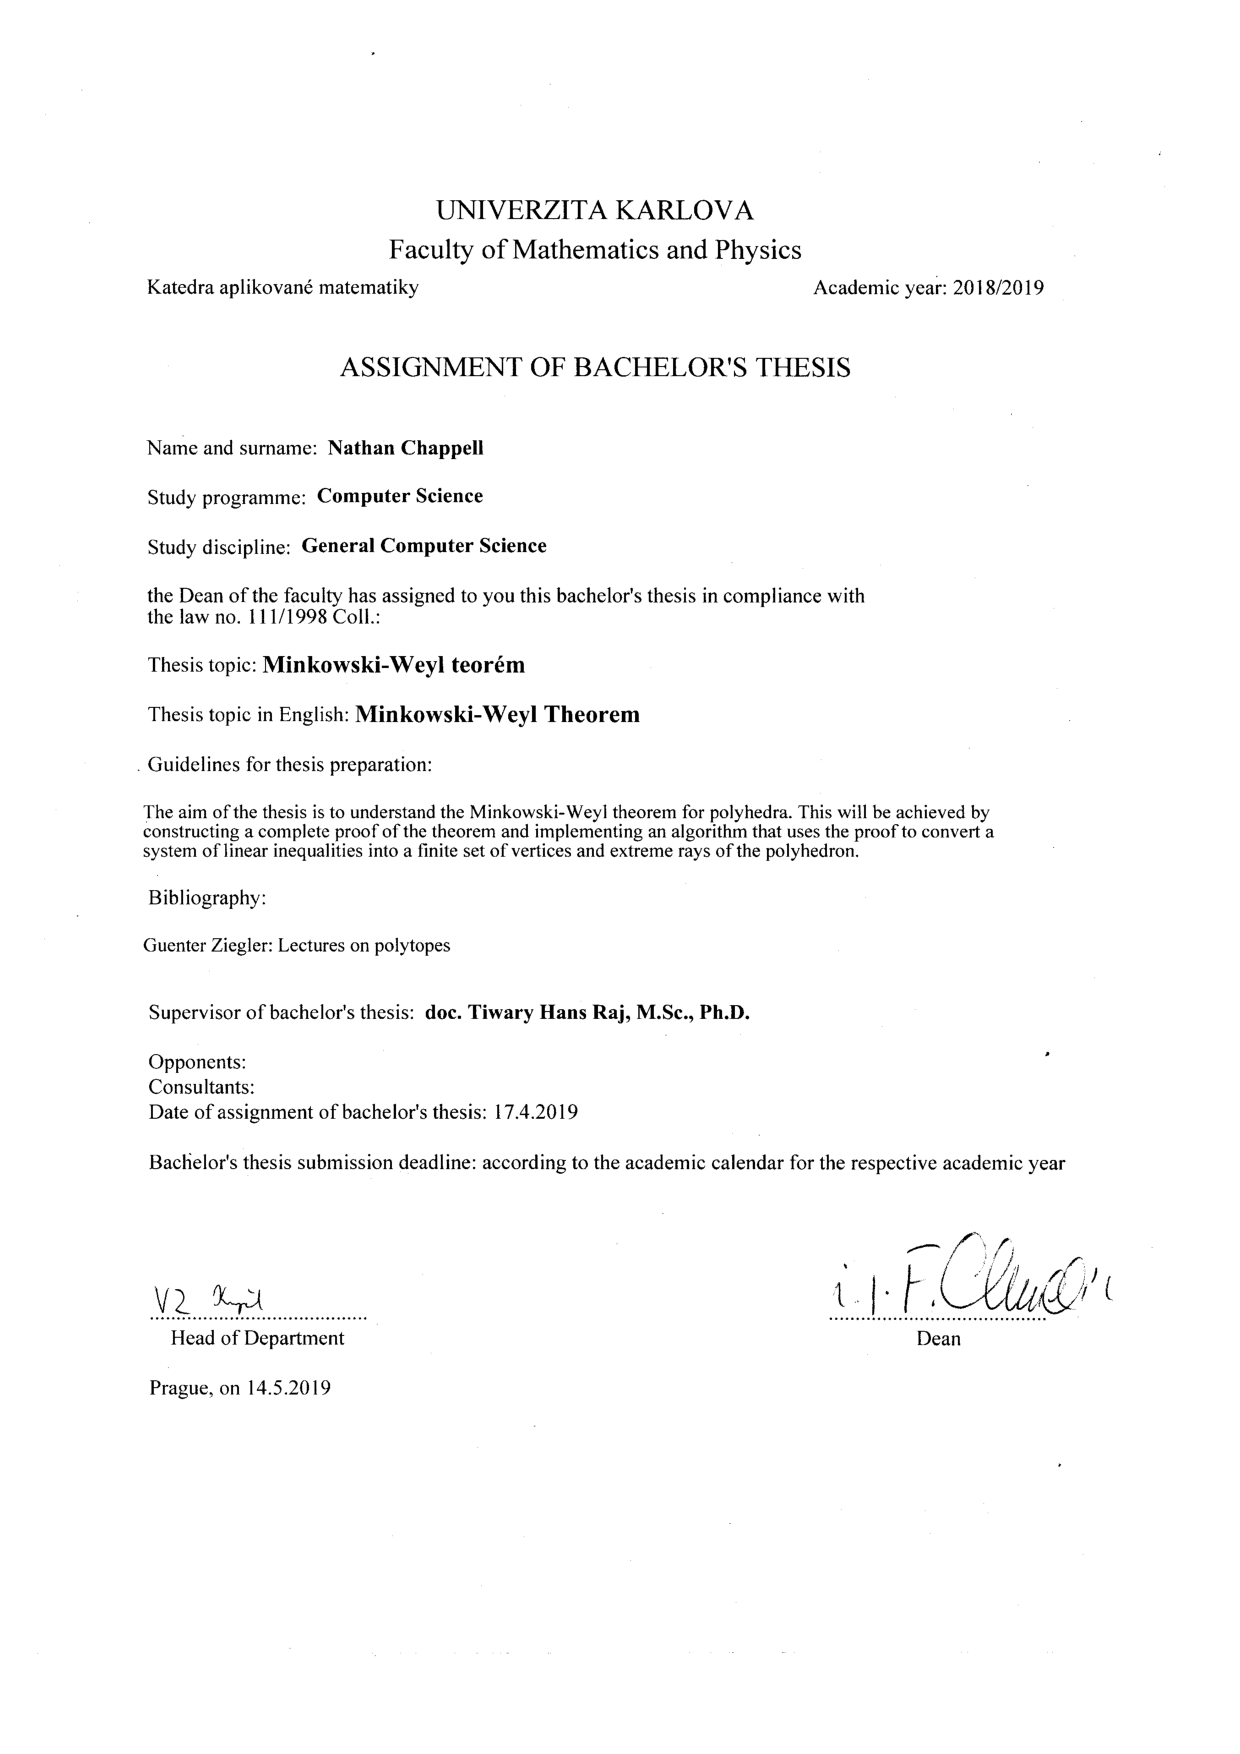
\includepdf{thesis_assignment.pdf}

%%%% Dedication
%
%\openright
%
%\noindent
%\Dedication
%
%\newpage
%
%%% Mandatory information page of the thesis

\openright

\vbox to 0.5\vsize{
\setlength\parindent{0mm}
\setlength\parskip{5mm}

Title:
\ThesisTitle

Author:
\ThesisAuthor

\DeptType:
\Department

Supervisor:
\Supervisor, \SupervisorsDepartment

Abstract:
\Abstract

Keywords:
\Keywords

\vss}

\newpage

\openright
\pagestyle{plain}
\pagenumbering{arabic}
\setcounter{page}{1}


%%% A page with automatically generated table of contents of the bachelor thesis

\tableofcontents

%%% Each chapter is kept in a separate file
\chapter*{Introduction}
\addcontentsline{toc}{chapter}{Introduction}

Polyhedra are fundamental mathematical objects.  Two ways of describing polyhedra are:
\begin{enumerate}
  \item A finite intersection of half-spaces
  \item The \textit{Minkowski-Sum} of the \textit{convex-hull} of a finite set of rays and a finite set of points
\end{enumerate}
The {\MWT} is a fundamental result in the theory of polyhedra.  It states that both means of representation are equivalent.  The proof given here is algorithmic in nature, using a technique known as \textit{Fourier-Motzkin elimination}.  The correctness of the algorithm also proves a result known as \nameref{farkas_lemma}.

This thesis is broken up into four chapters.  Chapter 1 states the definitions necessary for {\MWT}, and states the theorem.  Chapter 2 proves the theorem, by first considering the case that the polyhedron is a cone, then shows how to reduce the case of general polyhedra to that of cones.  Chapter 3 shows a C$++$ implementation of the transformations described in Chapter 2.  Chapter 4 presents a method of testing the program for special cases of polyhedra, known as either pointed or full-dimensional polyhedra.  \nameref{farkas_lemma} is proven and extensively used to show the validity of the testing methods.

\chapter{\MWT}

We begin somewhat tersely, stating some basic definitions in order to state the theorem.  The only noteworthy part of this section is \Cref{cone_closure}, which will be used a number of times throughout the paper.

\section{Polyhedra}

\begin{Def}[Non-negative Linear Combination]{
		Let $\mU$, $\tv$, ${\t \geq \0}$, then \( \tusum = U\t\) is called a \em{non-negative linear combination} of $U$.
	}\end{Def}

\begin{Def}[V-Cone]{
		Let $\mU$.  The set of all non-negative linear combinations of $U$ is denoted $\cone(U)$.  Such a set is called a \em{V-Cone}.
	}\end{Def}

\begin{Def}[Convex Combination]{
		Let $\mV$, and let $\lv$ satisfy $\lsum = 1$, $\l \geq\0$, then \( \lvsum \) is called a \textit{convex combination} of V.  The set of all convex combinations of $V$ is denoted $\conv(V)$.
	}\end{Def}

\begin{Def}[V-Polyhedron]{
		Let $\mV$, $\mU$.  Then the set
		%\[ \set{\tusum + \lvsum\St\,t_j \geq 0,\isconv} \]
		\[ \set{\x + \y \st \x \in \cone(U),\, \y \in \conv(V)} \]
		is called a \em{V-Polyhedron}.
	}\end{Def}

\paragraph{Note:} Given two sets $P$ and $Q$, the set $P+Q = \set{p+q\st p\in p,\,q\in Q}$ is called the \textit{Minkowski Sum} of $P$ and $Q$.  Therefore, we will write a V-Polyhedron as $\cone(U) + \conv(V)$ for some $U$ and $V$.\\

\begin{Def}[H-Polyhedron]{
		Let $\mA$, $\bv$.  Then the set
		\[ \set{\xv \St A\x \leq \b} \]
		is called an \em{H-Polyhedron}.
	}\end{Def}

\begin{Def}[H-Cone]{
		Let $\mA$. Then the set
		\[ \set{\xv \St A\x \leq \0} \]
		is called an \em{H-Cone}.
	}\end{Def}

A simple but useful property of cones is that they are closed under addition and positive scaling.

\begin{Prop}[Closure Property of Cones]\label{cone_closure}
	Let $C$ be either an H-Cone or a V-Cone, and for each $i$ let $\x^i \in C$, and $c_i \geq 0$.  Then:
	\[ \sumi c_i \x^i \in C \]
\end{Prop}

\begin{proof}
	First we prove Proposition \ref{cone_closure} for H-Cones, then for V-Cones.
	If, for each $i$, $A\x^i \leq \0$, then $A(c_i\x^i) = c_iA\x^i \leq \0$, and
	\[ A\left(\sumi c_i\x^i\right) = \sumi A (c_i\x^i) =
		\sumi c_i A\x^i \leq \sumi \0 \leq \0 \]
	So, $\sumi c_i\x^i \in C$ when $C$ is an H-Cone.  Next, suppose that $C = \cone(U)$, and for each $i$, $\exists \t_i \geq \0: \x^i = U\t_i$.  Then $c_i\t_i \geq \0$, and $\sumi c_i\t_i \geq \0$.  Therefore
	\[ \sumi c_i\x^i = \sumi c_i U\t_i = \sumi U(c_i\t_i)
		= U\left(\sumi c_i\t_i\right) \]
	So, $\sumi c_i\x^i \in C$ when $C$ is a V-Cone.
\end{proof}

This proposition will be used in the following way: if we wish to show that $\sumi c_i\x^i$ in a member of some cone $C$, it suffices to show that, for each $i$, $c_i \geq 0$ and $\x^i \in C$.

\begin{Remark}
\Cref{cone_closure} is a fundamental property of cones.  In fact, it could be used as an abstract definition of a cone, removed from geometric interpretation, then cones in euclidean space could be examined as important special classes.
\end{Remark}


\section{\MWT}

The following theorem is the basic result to be proved in this thesis, which states that V-Polyhedra and H-Polyhedra are two different representations of the same objects.

\begin{Thm}[{\MWT}]
		Every V-Polyhedron is an H-Poly-hedron, and every H-Polyhedron is a V-Polyhedron.
\end{Thm}

\chapter{Proof of the \MWT}

The proof proceeds by first showing that V-Cones are representable as H-Cones, and H-Cones are representable as V-Cones.  Then it is shown that the case of polyhedra can be reduced to cones.

%\begin{Thm}[{\MWT} for Cones] \label{MWTFC}
%  Every V-Cone is an H-Cone, and Every H-Cone is a V-Cone.
%\end{Thm}

\section{Every V-Cone is an H-Cone}

\begin{Thm} \label{MWTFCvtoh}
  Every V-Cone is an H-Cone.
\end{Thm}

To be clear, what we shall now show is that, given a set of the form: $\cone(U)$, there is an $A$ such that $\cone(U) = \HC{A}$.  The first step in this construction is to rewrite $\cone(U)$ as $\Pi\left(\HC{A'}\right)$, where $\Pi$ is a coordinate projection.  We then show how to calculate these projections, and that the result is a set of the form $\HC{A}$.

\begin{Def}[Coordinate Projection]
	Let $I$ be the identity matrix.  Then the matrix $I'$ formed by deleting some rows from $I$ is called a \textit{coordinate-projection}.
\end{Def}

\begin{Lemma}[Lifting a V-Cone]\label{vconelift}
	 Every V-Cone is a coordinate-projection of an H-Cone.
\end{Lemma}

\begin{Lemma}[Projecting an H-Cone]\label{hconeproject}
	 Every coordinate-projection of an H-Cone is an H-Cone.
\end{Lemma}

First, we quickly use the two lemmas to conclude \Cref{MWTFCvtoh}.  The rest of the section will be the proof of the two lemmas.

\begin{proof}[Proof of \Cref{MWTFCvtoh}]
	Given \Cref{vconelift} and \Cref{hconeproject}, the proof follows simply.  Given a V-Cone, we use \Cref{vconelift} to get a description involving coordinate-projection of an H-Cone.  Then we can apply \Cref{hconeproject} in order to get an H-Cone.
\end{proof}

\begin{proof}[Proof of \Cref{vconelift}]
	We prove that every V-Cone is a coordinate projection of an H-Cone, by giving an explicit formula.  Let ${\mU}$, and observe that
	\[ \cone(U) = \set{U\t \st \t \in \R^{\Udim},\, \t \geq \0} =
		\set{\xv \st (\exists \tv)\,\x = U\t,\, \t \geq \0} \]
	The plan is to express the equality of $U\t$ and $\x$ as two inequalities, and combine them in a block-matrix along with the non-negativity of $\t$, then project away the coordinates corresponding to $\t$.  The following expression takes one step:
	\begin{equation}\label{eq:tleqz}
		\t \geq \0 \Leftrightarrow -I\t \leq \0
	\end{equation}
	Using the equality: $a = 0 \Leftrightarrow a \leq 0 \land -a \leq 0$, and block matrix notation, we take the second step.
	\begin{equation}\label{eq:xeqt}
		\x = U\t \Leftrightarrow \x - U\t = \0 \Leftrightarrow
		\begin{pmatrix*}[r] I & -U \\ -I & U \end{pmatrix*} \xt \leq \0
	\end{equation}
	Comparing \eqref{eq:tleqz} and \eqref{eq:xeqt}, we define a matrix transform:
  \begin{Transform}[V-Cone Lift]\label{vconelift_transform}
  \[\VLift(U) = \pmb \0 & -I \\ I & -U \\ -I & U \pme \]
  \end{Transform}
  So we can rewrite $\cone(U)$:
	\begin{equation*}
		\cone(U) = \set{ \xv \St \VLift(U)\xt \leq \0}
	\end{equation*}
	Let $\Pi$ be the identity matrix in $\R^{(d+\Udim)\times(d+\Udim)}$, but with the last $\Udim$-rows deleted.  Then $\Pi$ is a coordinate projection, and the above expression can be written:
	\begin{equation}\label{eq:vconelift}
		\cone(U) = \Pi\left(\set{ \y \in \R^{d+\Udim} \st \VLift(U)\y \leq \0}\right)
	\end{equation}
	This is a coordinate projection of an H-Cone, and \Cref{vconelift} is shown.
\end{proof}

To prove \Cref{hconeproject}, we use two separate propositions.
\begin{Prop}[Projecting Null Columns]\label{proj_0_columns}
	Let $B\in\R^{m\times(d+\Udim)}$, with the last $\Udim$ columns all $\0$.  Let $B'$ be $B$ with the last $\Udim$ columns deleted, and $\Pi$ the identity matrix in $\R^{d+\Udim}$ with the last $\Udim$ rows deleted.  Then
	\[ \Pi\left(\set{\y \in \R^{d+\Udim} \st B\y \leq \0}\right) =
		\set{\x\in\R^d\st B'\x\leq\0} \]
\end{Prop}

\begin{proof}
	Recall that $B\y \leq \0$ means that $(\forall i)\ip{B_i}{\y} \leq 0$.  Because the last $\Udim$ columns of $B$ are $\0$, any row $B_i$ of $B$ can be written $(B'_i,\0)$, with $\0 \in \R^\Udim$.  We can also rewrite $\y\in\R^{d+\Udim}$ as $(\x,\w)$ with $\x\in\R^d,\w\in\R^\Udim$, so that $\x = \Pi(\y)$.  Then
	\[ \ip{B_i}{\y} = \ip{(B'_i,\0)}{(\x,\w)} = \ip{B'_i}{\x} = \ip{B'_i}{\Pi(\y)} \]
	It follows that
	\[ \ip{B_i}{\y} \leq 0 \Leftrightarrow \ip{B'_i}{\Pi(\y)} \leq 0 \]
	Since $B_i$ is an arbitrary row of $B$, the proposition is shown.
\end{proof}

In order to use the above proposition, we need a matrix with columns which are $\0$.  The next proposition shows us how to obtain such a matrix from another, while maintaining certain important properties.

\begin{Prop}[Fourier Motzkin Elimination for H-Cones]\label{fm_hcone}
	Let ${\mB}$.  Then there exists a matrix $\mC$ with the following properties:
	\begin{enumerate}
		\item Every row of $B'$ is a positive linear combination of rows of $B$.
		\item $m_2$ is finite.
		\item The $k$-th column of $B'$ is $\0$.
		\item \((\exists t)B(\x + t\e_k) \leq \0 \Leftrightarrow B'\x \leq \0\)
	\end{enumerate}
\end{Prop}

\begin{proof}
	Partition the rows of $B$ as follows:
	\begin{alignat*}{3}
		 & P &  & = i & \st & \Bik > 0 \\
		 & N &  & = j & \st & \Bjk < 0 \\
		 & Z &  & = l & \st & \Blk = 0
	\end{alignat*}
	Then let $B'$ be a matrix with the following rows:
	\begin{alignat*}{3}
		 & B'_l    &  & = B_l                 & \st & l \in Z          \\
		 & B'_{ij} &  & = \Bik B_j - \Bjk B_i & \st & i \in P, j \in N
	\end{alignat*}
	\textit{1} and \textit{2} are clear.  \textit{3} is satisfied for rows indexed by $Z$ by definition  That it holds for the other rows, observe:
   \[\ip{B'_{ij}}{\e_k} = \ip{\Bik B_j - \Bjk B_i}{\e_k} = \Bik \Bjk - \Bjk \Bik = 0\]
	The right direction of \textit{4} is shown in the following calculations.  Because $\Blk = 0$:
	\[ \ip{B_l}{\x+t\e_k} = \ip{B_l}{\x} + t\Blk = \ip{B_l}{\x} = \ip{B'_l}{\x} \]
	So $\ip{B_l}{\x+t\e_k} \leq 0 \Leftrightarrow \ip{B'_l}{\x} \leq 0$.  It follows that \textit{4} is satisfied for rows indexed by $Z$, and we will turn to rows indexed by $P$ and $N$. Because $\Bik \Bjk - \Bjk \Bik = 0$ we have:
	\[ \ip{\Bik B_j - \Bjk B_i}{\x + t\e_k} = \ip{\Bik B_j - \Bjk B_i}{\x} \]
	Because $\Bik$ and $-\Bjk$ are non-negative:
	\[ \ip{B_i}{\x+t\e_k} \leq 0,\; \ip{B_j}{\x+t\e_k} \leq 0 \Rightarrow
		\ip{\Bik B_j - \Bjk B_i}{\x + t\e_k} \leq 0\]
	Therefore $\ip{\Bik B_j - \Bjk B_i}{\x} \leq 0$, and the right implication is shown.

	Now suppose that $B'\x \leq \0$.  The task is to find a $t$ so that $B(\x+t\e_k)\leq \0$.  Observe
	\begin{alignat*}{3}
		\faij & \quad & \ip{\Bik B_j - \Bjk B_i}{\x}    & \leq  \; 0                                & \Leftrightarrow \\
		\faij & \quad & \ip{\Bik B_j}{\x}               & \leq  \; \ip{\Bjk B_i}{\x}                & \Leftrightarrow \\
		\faij & \quad & \ip{B_i/\Bik}{\x}               & \leq  \; \ip{B_j/\Bjk}{\x}                & \Leftrightarrow \\
		      & \quad & \max_{i\in P} \ip{B_i/\Bik}{\x} & \leq  \; \min_{j\in N}  \ip{B_j/\Bjk}{\x} &
	\end{alignat*}
	Note that the third inequality changes directions because $\Bjk < 0$.  Now we choose $t$ to lie in this last interval, and show that we can use it to satisfy all of the constraints given by $ B$.  So, we have a $t$ such that
	\[ \max_{i\in P} \ip{B_i/\Bik}{\x} \leq t \leq \min_{j\in N} \ip{B_j/\Bjk}{\x} \]
	In particular,
  \[(\forall j\in N)\quad t \leq \ip{B_j/\Bjk}{\x} \Rightarrow \ip{B_j}{\x} - \Bjk t \leq 0\]
	Again, the inequality changes directions because $\Bjk < 0$.  Now consider a row $ B_j$ from $ B$:
	\[ \ip{B_j}{\x-t\e_k} =  \ip{B_j}{\x} - \Bjk t \leq 0 \]
	Similarly,
  \[(\forall i\in P)\quad \ip{B_i/\Bik}{\x} \leq t \Rightarrow \ip{B_i}{\x} - \Bik t \leq 0 \]
	Now consider a row $ B_i$ from $ B$:
	\[ \ip{B_i}{\x-t\e_k} =  \ip{B_i}{\x} - \Bik t \leq 0 \]
	So, we've demonstrated that $\x-t\e_k$ satisfies all the constraints from $B$, and the left implication is shown.  So \textit{4} holds.
\end{proof}

\begin{Remark}[Fourier Motzkin Matrix]\label{fm_matrix}
	 \Cref{fm_hcone} highlights the properties of the matrix $B'$.  Upon close inspection, we can create a Matrix $Y$ such that $B' = YB$, and every element of $Y$ is non-negative.  Create the following set of row vectors $Y$
	\begin{alignat*}{2}
		 & \e_l                  & \st & l \in Z          \\
		 & \Bik \e_j - \Bjk \e_i & \st & i\in P,\; j\in N
	\end{alignat*}
	Since the basis vectors simply select rows during matrix multiplication, it is clear that
	\[ B' = YB \]
\end{Remark}

\begin{proof}[Proof of \Cref{hconeproject}]
	Here we prove the case that the coordinate projection is onto the first $d$ of $d+p$ coordinates.  Let $\set{\y\in\R^{d+\Udim}:A'\y \leq \0}$ be the H-Cone we need to project, and $\Pi$ the coordinate-projection we need to apply (the identity matrix with the last p rows deleted).  For each $1 \leq k \leq p$ we can use \Cref{fm_hcone} in an incremental manner, starting with $A'$.
	\begin{align*}
		 & \text{let } B_0 := A'                                        \\
		 & \text{for } 1 \leq k \leq p                                  \\
		 & \quad \text{let } B_k :=
		\text{result of proposition 2 applied to $B_{k-1}$, $\e_{d+k}$} \\
		 & \text{endfor}                                                \\
		 & \text{return } B_p
	\end{align*}

	Consider the resulting $B$.  Property \textit{2} holds throughout, so $B$ is finite.  After each iteration, property \textit{3} holds for $d+k$, so the $(d+k)$-th column is $\0$.  Since each iteration only results from non-negative combinations of the result of the previous iteration (property \textit{1}), once a column is $\0$ it remains so.  Therefore, at the end of the process, the last $p$ columns of $B$ are all $\0$.  Then, by \Cref{proj_0_columns}, we can apply $\Pi$ to $B$ by simply deleting the last $p$ columns of $B$.  Denote this resulting matrix $A$.  We still need to check that
	\begin{equation}\label{eq:V2equal}
		\Pi\set{\y\in\R^{d+\Udim}\st A'\y\leq\0} = \set{\x\in\R^{d}\st A\x\leq\0}
	\end{equation}
	This follows from the following:
	\begin{align}
		A'\y & \leq \0 \Rightarrow A(\Pi(\y)) \leq \0 \label{V2seteqright}                                                           \\
		A\x  & \leq \0 \Rightarrow (\exists t_1)\dots(\exists t_p) A'(\x+t_1\e_{d+1}+\cdots+t_p\e_{d+p}) \leq \0 \label{V2seteqleft}
	\end{align}
	The key observation of this verification utilizes property \textit{4} of \Cref{fm_hcone}:
	\[ (\exists t)B(\x + t\e_k) \leq \0 \Leftrightarrow B'\x \leq \0 \]
	In what follows, let $\x = \sum_{1 \leq j \leq d}x_j\e_j$.  The above property is applied sequentially to the sets $B_k$ as follows:
	\begin{alignat*}{2}
		(\exists t_p)(\exists t_{p-1})\dots(\exists t_1)                & \quad
		B_0(\x + t_1\e_{p} + t_2\e_{p-1} + \dots + t_p\e_{d}) \leq \0\; & \Leftrightarrow                                                 \\
		(\exists t_p)\dots(\exists t_2)                                 & \quad
		B_1(\x + t_2\e_{d+2} + \dots + t_p\e_{d+p})
		\leq \0                                                         & \Leftrightarrow                                                 \\
		\vdots \hspace{1.3em}                                           & \hspace{5em}\vdots                       & \vdots\hspace{0.4em} \\
		(\exists t_p)                                                   & \quad B_{p-1}(\x + t_p\e_{d+p})  \leq \0 & \Leftrightarrow      \\
		                                                                & \quad B_{p}\x  \leq \0                   &
	\end{alignat*}
	Because $A' = B_0$, and $A$ is $B_p$ with the last $p$ columns deleted, \eqref{V2seteqright} and \eqref{V2seteqleft} hold, therefore \eqref{eq:V2equal} holds, and the proof of \Cref{hconeproject} is complete, and we've shown that a coordinate projection of an H-Cone is again an H-Cone.
\end{proof}

With \Cref{vconelift} and \Cref{hconeproject} proven, we are now certain that every V-Cone is also an H-Cone.

\section{Every H-Cone is a V-Cone}

\begin{Thm} \label{MWTFChtov}
  Every H-Cone is a V-Cone.
\end{Thm}

Now we suppose that we are given a set of the form $\HC{A}$, and we must show that there is some $U$ such that $\cone(U) = \HC{A}$.  In a manner similar to the previous section, we will first write the set $\HC{A}$ as an intersection of a set $\cone(U')$ with a number of hyperplanes, then give a process to get rid of those intersections.

\begin{Def}[Coordinate Hyperplane]
	A set of the form
	\[ \set{\x \in \R^{\Adim} \st \ip{\x}{\e_k} = 0} =
		\set{\x \in \R^{\Adim} \st x_k = 0}
	\]
	is called a \em{coordinate-hyperplane}.
\end{Def}

This is how coordinate hyperplanes will be used.  We consider a V-Cone intersected with some coordinate hyperplanes, and write it in the following way:
\begin{equation}\label{eq:coneintform1}
	\set{\xv \St (\exists \t \geq 0) \xz = U'\t}
\end{equation}
If we suppose that $U' \subset \R^{d+\Adim}$, and $\Pi$ is the identity matrix with the last $\Adim$ rows deleted, then this is just a convenient way of writing:
\begin{equation}\label{eq:coneintform2}
	\Pi\big(\cone(U') \cap \set{x_{d+1} = 0}
	\cap \dots \cap \set{x_{d+\Adim} = 0}\big)
\end{equation}
The proof that every H-Cone is a V-Cone rests on the following three propostions:
\begin{Lemma}[Lifting an H-Cone]\label{hconelift}
  Every H-Cone is a coordinate-projection of a V-Cone intersected with some coordinate hyperplanes.
\end{Lemma}
\begin{Lemma}[Intersecting a V-Cone]\label{vconeintersect}
  Every V-Cone intersected with a coordinate-hyperplane is a V-Cone.
\end{Lemma}
\begin{Lemma}[Projecting a V-Cone]\label{vconeproject}
  Every coordinate-projection of a V-Cone is a V-Cone.
\end{Lemma}

We quickly dispatch \Cref{MWTFChtov} with these lemmas, then get to the real work of proving the lemmas.

\begin{proof}[Proof of \Cref{MWTFChtov}]
	Given \Cref{hconelift}, \Cref{vconeintersect}, and \Cref{vconeproject}, the proof follows simply.  Given an H-Cone, we use \Cref{hconelift} to get a description involving the coordinate-projection of a V-Cone intersected with some coordinate-hyperplanes.  We apply \Cref{vconeintersect} as many times as necessary to eliminate the intersections, then we can apply \Cref{vconeproject} in order to get a V-Cone.
\end{proof}

\begin{proof}[Proof of \Cref{hconelift}]
	Let $\mA$, we now show that the H-Cone
	\[\set{\xv \st A\x \leq \0}\]
	can be written as the projection of a V-Cone intersected with some hyperplanes.  We use the following transform.
  \begin{Transform}[H-Cone Lift]\label{hconelift_transform}
  \[\HLift(A) = \pmb \0 & I & -I \\ I & A & -A \pme \]
  \end{Transform}
  In other words,
  \[\HLift(A) =  \set{\zei, \eAj, \neAj, 1 \leq j \leq d,\, 1 \leq i \leq m}\]
	We then claim:
	\begin{equation}\label{eq:hliftform}
		\set{\xv \st A\x \leq \0} = \set{\xv \St (\exists \t \geq 0) \xz = \HLift(A)\t}
	\end{equation}
	First, considering \eqref{eq:coneintform1} and \eqref{eq:coneintform2}, observe that this is a coordinate-projection of a V-Cone intersected with some coordinate-hyperplanes.
	Next, we note that
	\[ \xAx = \jsum x_j \eAj \]
	We can write this as a sum with all positive coefficients if we split up the $x_j$ as follows:
	\[
		\xjp = \begin{cases} x_j & x_j \geq 0 \\ 0 & x_j < 0 \end{cases} \quad\quad\quad
		\xjm = \begin{cases} 0 & x_j \geq 0 \\ -x_j & x_j < 0 \end{cases}
	\]
	Then we have
	\begin{equation} \label{eq:xAx}
		\xAx = \jsum \xjp \eAj + \jsum \xjm \neAj
	\end{equation}
	where $\xjp, \xjm \geq 0$.  Also observe that
	\[ A\x \leq \0 \Leftrightarrow (\exists \w \geq \0) \st A\x + \w = \0 \]
	This can be written
	\begin{equation} \label{eq:Axz}
		A\x \leq \0 \Leftrightarrow (\exists \w \geq \0) \St \xAx + \zw = \xz
	\end{equation}
	\eqref{eq:xAx} and \eqref{eq:Axz} together show
	\[ A\x \leq \0 \Rightarrow (\exists \t \geq 0) \xz = \HLift(A)\t \]
	Conversely, suppose
	\[ (\exists \t \geq 0) \xz = \HLift(A)\t \]
	We would like to show that $A\x \leq \0$.  Let $\xjp,\xjm,w_i$ take the values of $\t$ that are coefficients of $\eAj$, $\neAj$, and $\zei$ respectively, and denote $x_j = \xjp - \xjm$.  Then we have
	\begin{align*}
		\xz & = \jsum \xjp \eAj + \jsum \xjm \neAj + \isum w_i\zei \\
		    & = \jsum x_j \eAj + \isum w_i\zei                     \\
		    & = \xAx + \zw
	\end{align*}
	where $\w \geq \0$.  By \eqref{eq:Axz} we have $A\x \leq \0$.  So \eqref{eq:hliftform} holds.
\end{proof}

The proof of \Cref{vconeintersect} relies upon the following proposition.
\begin{Prop}[Fourier Motzkin Elimination for V-Cones]\label{fm_vcone}
	Let ${Y \in \R^{(d+m)\times n_1}}$, $1 \leq k \leq d+m$, and $\x$ satisfy $x_k = 0$.  Then there exists a matrix $Y' \in \R^{(d+m)\times n_2}$ with the following properties:
	\begin{enumerate}
		\item Every column of $Y'$ is a positive linear combination of columns of $Y$.
		\item $n_2$ is finite.
		\item The $k$-th row of $Y'$ is $\0$.
		\item \((\exists \t\geq\0)\;\x = Y\t \Leftrightarrow (\exists \t' \geq \0)\;\x = Y'\t'\)
	\end{enumerate}
\end{Prop}

\begin{proof}
	We partition the columns of $ Y$:
	\begin{alignat*}{3}
		 & P &  & = i \; & \st & \Yi > 0 \\
		 & N &  & = j \; & \st & \Yj < 0 \\
		 & Z &  & = l \; & \st & \Yl = 0
	\end{alignat*}
	We then define $ Y'$:
	\[  Y' = \set{ Y^l \st l \in Z} \cup
		\set{\Yi Y^j - \Yj Y^i \st i \in P,\, j\in N} \]
	\textit{1} and \textit{2} are clear.  \textit{3} can be seen from:
	\begin{align}
		\ip{Y'^l}{\e^k}    & = 0 \nonumber                                                                \\
		\ip{Y'^{ij}}{\e^k} & = \ip{\Yi Y^j - \Yj Y^i}{\e^k} = \Yi \Yj - \Yj \Yi = 0 \label{eq:hdropZrows}
	\end{align}

	The left direction of \textit{4} follows from observing that a positive linear combination of positive linear combinations is again a positive linear combination.  Before moving on to the proof of the right direction of \textit{4}, we first note how we may write our vectors.
	\[  Y\t = \Zsum t_l  Y^l + \Psum t_i  Y^i + \Nsum t_j  Y^j \]
	\[  Y'\t = \Zsum t_l  Y^l + \NPsum t_{ij} (\Yi Y^j - \Yj Y^i) \]
	Then, by \nameref{cone_closure}, to show that the proposition is true, we need only show that, given some $t_i, t_j \geq 0$ satisfying $\Psum t_i  Y^i_{k} + \Nsum t_j  Y^j_{k} = 0$, there exists $t_{ij} \geq 0$ such that
	\begin{equation} \label{eq:coneEq}
		 \Psum t_i  Y^i + \Nsum t_j  Y^j = \NPsum t_{ij} (\Yi Y^j - \Yj Y^i)
	\end{equation}

	\newcommand{\coneEqSat}{\quad\mathrm{\;such\; that\; \eqref{eq:coneEq}\; holds}}
		First note that if all $t_i = 0,t_j = 0$, then choosing $t_{ij} = 0$ satisfies \eqref{eq:coneEq}.  So suppose that some $t_i \neq 0, t_j \neq 0$.  Observe:
		\[ 0 = \Psum t_i\Yi + \Nsum t_j\Yj \Rightarrow \Psum t_i\Yi = -\Nsum t_j\Yj\]
		Denote the value in this equality as $\sigma$, and note that $\sigma > 0$.  Then
		\begin{alignat*}{3}
			\Psum t_i Y^i & = & \frac{-\Nsum t_j \Yj}{\sigma}\Psum t_i Y^i & =
			\NPsum -\frac{t_i t_j}{\sigma}\Yj Y^i                              \\
			\Nsum t_j Y^j & = & \frac{\Psum t_i \Yi}{\sigma}\Nsum t_j Y^j  & =
			\NPsum \frac{t_i t_j}{\sigma}\Yi Y^j
		\end{alignat*}
		Combining these results, we have
		\[ \Psum t_i Y^i + \Nsum t_j Y^j = \NPsum \frac{t_i t_j}{\sigma}(\Yi Y^j - \Yj Y^i) \]

	Finally, we can conclude that, given $\t \geq \0$, if $Y\t$ has a $0$ in the $k$-th coordinate, then we can write it as $ Y'\t'$ where $\t' \geq \0$, and any non-negative linear combination of vectors from $Y'$ can be written as a non-negative linear combination of vectors from $Y$, and will necessarily have the $k$-th coordinate be $0$ by property \textit{3}.  So property \textit{4} holds.
\end{proof}

\begin{proof}[Proof of \Cref{vconeintersect}]
	In \Cref{fm_vcone}, the assumption that $x_k = 0$ in property \textit{4} creates the set $\cone(Y) \cap \set{\x \st x_k = 0}$.  This set, by property \textit{4}, is $\cone(Y')$.
\end{proof}

\begin{proof}[Proof of \Cref{vconeproject}]
	We shall prove that the coordinate-projection of a V-Cone is again a V-Cone.  Let $\Pi$ be the relevant projection, then we have:
	\[ \Pi\set{U\t \st \t \geq \0} = \set{\Pi(U\t) \st \t \geq \0} =
		\set{(\Pi U)\t \st \t \geq \0} \]
	The last equality follows from associativity of matrix multiplication.  Therefore,
	\[ \Pi\big(\cone(U)\big) = \cone\big(\Pi U\big) \]
\end{proof}

The final step, as in the previous section, is to show that the iterative process of intersecting a V-Cone with coordinate hyperplanes iteratively yields V-Cones.  This is merely applying \Cref{fm_vcone} multiple times, so the details are omitted.  Having shown that H-Cones are V-Cones, the proof of the {\MWT} for cones is complete.

\section{Reducing Polyhedra to Cones}

\subsection{H-Polyhedra $\to$ V-Polyhedra}

The transformation of an H-Polyhedron goes as follows:
\begin{align*} 
\{\x\st A\x\leq\b\}
    &= \Pi\left(\left\{
      [-\b|A]\xx\leq\0\right
      \}\cap\hpxz\right) \\
    &= \Pi\left(\cone(U')\cap\hpxz\right)\\ 
    &= \Pi\left(\cone\pmb \0 & \1 \\ U & V\pme \cap\hpxz\right)\\
    &= \cone(U) + \conv(V)
\end{align*}

The first equality can be seen by inspection.  The second equality is given by \Cref{MWTFChtov}.  The fourth inequality isn't hard to see -- just note that for $x_0$ to be equal to $1$ a convex combination of the vectors from $\psmb\1\\ V\psme$ must be taken.  The third equality requires some work.

\begin{Prop}[V-Cone $\to$ V-Polyhedron]\label{vcone_to_vpoly}
	Given some $U'$, precisely one of the following two statements holds:
	\begin{align*}
    (\exists U,V)\;&\cone(U') \cap \hpxz = 
        \cone\pmb \0 & \1 \\ U & V \pme \cap \hpxz \\
  &\cone(U') \cap \hpxz \text{ is empty}
  \end{align*}
\end{Prop}

\begin{proof}
  The second case may occur if there are no elements of $U'$ with $x_0 > 0$.  Otherwise, we partition $U'$ into the sets:
	\begin{alignat*}{3}
		 & P &  & = i & \st & \Uiz > 0 \\
		 & N &  & = j & \st & \Ujz < 0 \\
		 & Z &  & = l & \st & \Ulz = 0
	\end{alignat*}
	And define two new sets:
	\begin{align*}
		\bar U   & = \set{U^l \st l \in Z} \cup \set{\Uiz U^j - \Ujz U^i \st i\in P,\, j\in N} \\
		\bar V\; & = \set{U^i/\Uiz \st i \in P}
	\end{align*}
  Let $U$ and $V$ be $\bar U$ and $\bar V$ with the first row deleted, respectively (i.e. $\bar U = \psmb\0\\ U\psme$, and $\bar V = \psmb\1\\ V\psme$.  Then I claim that
	\[ \cone(U) \cap \hpxz = \cone\pmb \0 & \1 \\ U & V \pme \cap \hpxz\]
  Clearly $\cone\psmb \0 & \1 \\ U & V \psme \subseteq \cone(U)$, because the cone on the left is generated by elements of the one on the right.  Suppose that $\z \in \cone(U) \cap \shpxz$, then $\z$ can be written
	\[ \z = \Zsum t_l U^l + \Psum t_i U^i + \Nsum t_j U^j \]
	It will be convenient to use shorter notation for these sums.  Define the following:
	\begin{alignat*}{3}
		\bsigma_Z & = \Zsum t_l U^l, \quad &  & \sigma_l \, & = & \, \Zsum t_l \Ulz \;= 0 \\
		\bsigma_P & = \Psum t_i U^i, \quad &  & \sigma_i \, & = & \, \Psum t_i \Uiz       \\
		\bsigma_N & = \Nsum t_j U^j, \quad &  & \sigma_j \, & = & \, \Nsum t_j \Ujz
	\end{alignat*}
	Then it holds that
	\[ \ip{\e_0}{\z} = \sigma_l + \sigma_i + \sigma_j = \sigma_i + \sigma_j = 1
		\quad\Rightarrow\quad -\sigma_j/\sigma_i = 1 - 1/\sigma_i \]
	\[ \bsigma_P = \bsigma_P/\sigma_i + (1-1/\sigma_i)\bsigma_P
		= \bsigma_P/\sigma_i - (\sigma_j/\sigma_i)\bsigma_P \]
	Using the new notation, we can rewrite $\z$:
	\[ \z = \bsigma_Z + \bsigma_P + \bsigma_N
		= \bsigma_Z + \frac{\bsigma_P}{\sigma_i} - \frac{\sigma_j}{\sigma_i}\bsigma_P
		+ \frac{\sigma_i}{\sigma_i}\bsigma_N
		= \bsigma_Z + \frac{\bsigma_P}{\sigma_i} +
		\frac{\sigma_i\bsigma_N - \sigma_j\bsigma_P}{\sigma_i}
	\]
  And now it's fairly clear that $\z \in \cone\psmb \0 & \1 \\ U & V \psme$.
\end{proof}

\subsection{V-Polyhedra $\to$ H-Polyhedra}

The generalization in this direction is considerably simpler:

\begin{align*} 
\cone(U) + \conv(V)
    &= \Pi\left(\cone\pmb \0 & \1 \\ U & V\pme \cap\hpxz\right)\\
    &= \Pi\left(\left\{
      [-\vec{b}|A]\xx\leq\0\right
      \}\cap\hpxz\right) \\
    &= \{\x\st A\x\leq\vec{b}\}
\end{align*}

The first equality follows from the discussion in the previous section.  The second equality is \Cref{MWTFCvtoh}, written in a particularly ugly way to single out the first column of the constraint matrix.  The third equality follows again from inspection.

\section{Picture of the Proof}
Here we show a diagram that represents the proof of the {\MWT}.
\definecolor{mygrey}{rgb}{.1,.1,.1}
\newcommand{\FIGstep}{2}
\newcommand{\FIGge}{8}
\newcommand{\FIGgd}{\numexpr \FIGge-\FIGstep}
\newcommand{\FIGgc}{\numexpr \FIGgd-\FIGstep}
\newcommand{\FIGgb}{\numexpr \FIGgc-\FIGstep}
\newcommand{\FIGga}{\numexpr \FIGgb-\FIGstep}
\newcommand{\ptovcolor}{violet}
\newcommand{\liftcolor}{blue}
\newcommand{\dropcolor}{red}
\newcommand{\VDropdesc}{$\Pi\circ\bigcap$}
\newcommand{\HDropdesc}{$\Pi$}
\newcommand{\HPdesc}{\HP{A}{\b}}
\newcommand{\HPidesc}{\LHC}
\newcommand{\HCdesc}{\HC{A}}
\newcommand{\HCpdesc}{\pmb \0 & -I \\ I & -U \\ -I & U \pme \x \leq \0}
\newcommand{\VPdesc}{\VP{U}{V}}
%\newcommand{\VPidesc}{\cone\{\smallstack{\vec{0}}{U}\cup\smallstack{\vec{1}}{V}\}}
\newcommand{\VPidesc}{\cone\pmb\vec{0}&\vec{1}\\{U}&{V}\pme}
\newcommand{\VCdesc}{\cone(U)}
\newcommand{\VCpdesc}{\cone \pmb 0 & I & -I\\ I & A & -A\pme}
\begin{figure}[H]
	\begin{centering}
  %\leavevmode\beginpgfgraphicnamed{jobProofFlowChart}
		\begin{tikzpicture}[>=triangle 45]
			\node (HP)  at (\FIGgd,\FIGge) {\framebox{$\HPdesc$}};
			\node (HPi) at (\FIGga,\FIGge) {\framebox{$\HPidesc$}};
			\node (HC)  at (\FIGga,\FIGgc) {\framebox{$\HCdesc$}};
			\node (HCp) at (\FIGgc,\FIGgb) {\framebox{$\HCpdesc$}};
			%
			\node (VP)  at (\FIGgb,\FIGga) {\framebox{$\VPdesc$}};
			\node (VPi) at (\FIGge,\FIGga) {\framebox{$\VPidesc$}};
			\node (VC)  at (\FIGge,\FIGgc) {\framebox{$\VCdesc$}};
			\node (VCp) at (\FIGgc,\FIGgd) {\framebox{$\VCpdesc$}};
			\draw[<->,color=\ptovcolor] (HP) to node[below]{lift} node[above]{\HDropdesc} (HPi);
			\draw[<->,color=\ptovcolor] (VP) to node[above]{lift} node[below]{\VDropdesc} (VPi);
			\draw[-,dashed,color=mygrey]  (HPi) to node[rotate=90,above]{(relabel)} (HC);
			\draw[-,dashed,color=mygrey]  (VPi) to node[rotate=90,below]{(relabel)} (VC);
			\draw[->,color=\liftcolor,bend left] (HC)  to node[above left]{lift} (VCp);
			\draw[->,color=\dropcolor,bend left] (VCp) to node[above right]{\VDropdesc} (VC);
			\draw[->,color=\liftcolor,bend left] (VC)  to node[below right]{lift} (HCp);
			\draw[->,color=\dropcolor,bend left] (HCp) to node[below left]{\HDropdesc} (HC);
			%HP <-> HPi
			%VP <-> VPi
			%HPi -  HC
			%VPi -  VC
			%HC  -> VCp
			%VC  -> HCi
			%VCp -> VC
			%HCp -> HC
			%
			%HPi  <-> HP
			%|
			%| ____VCp___
			%HC_        _VC
			%   \__HCp_/ |
			%            |
			%   VP <->  VPi
		\end{tikzpicture}
    %\endpgfgraphicnamed
		\caption{Diagram of the proof $P_H \leftrightarrow P_V$}
		\label{fig:h_to_v}
	\end{centering}
\end{figure}

Figure \ref{fig:h_to_v} shows the flow from an H-Polyhedron to a V-Polyhedron and back.  There are \textcolor{\ptovcolor}{{\ptovcolor} arrows} for transformations back and forth from polyhedra to cones, \textcolor{\liftcolor}{{\liftcolor} arrows} to show the transformation between cones and intermediate representations, and \textcolor{\dropcolor}{{\dropcolor} arrows} to show where Fourier Motzkin elimination is applied to reduce these intermediate representations to standard cones.  V-Cones are \textcolor{\liftcolor}{lifted} to H-Cones which need to be \textcolor{\dropcolor}{projected (\HDropdesc)}, and H-Cones are \textcolor{\liftcolor}{lifted} to V-Cones which need to be \textcolor{\dropcolor}{intersected and projected (\VDropdesc)}.
 
\chapter{C++ Implementation}
%TODO update the content below, migrate commentary, input usage file...

The above transformations have been implemented in C++.  Program \lsti{main.cpp} takes one argument specifying the type of input object.  It reads the description of the object from standard input, and writes the result of the implied transformation to standard output.  If no arguments are supplied, then a \lsti{usage} message is given.  The \lsti{usage} message, which also contains the input format for the objects, is:

\VerbatimInput{../../usage.txt}

The files pertaining to the implementation will be discussed in the following sections, but here is a table showing the include dependencies followed by a short summary of the files. \\

\begin{tabular}{|l|l|}
	\hline
	file                          & includes                                             \\
	\hline
	\filename{linear\_algebra.h}  &                                                      \\
	\filename{fourier\_motzkin.h} & \filename{linear\_algebra.h}                         \\
	\filename{polyhedra.h}        & \filename{fourier\_motzkin.h}                        \\
	\filename{main.cpp}           & \filename{polyhedra.h}                               \\
	\filename{test\_functions.h}  & \filename{linear\_alebra.h}                          \\
	\filename{test.cpp}           & \filename{test\_functions.h}, \filename{polyhedra.h} \\
	\hline
\end{tabular}\\

\vspace{1em}

Here is a very brief summary of the files mentioned in the above table, more details are given in sequent sections.

\begin{itemize}
	\item \texttt{linear\_algebra.h} \\
	      Types \lsti{Vector} and \lsti{Matrix}, and some basic functionality for them
	\item \texttt{fourier\_motzkin.h} \\
	      Fourier Motzkin elimination, {\MWT} for cones
	\item \texttt{polyhedra.\{cpp,h\} } \\
	      Transforms between polytopes and polyhedra, {\MWT}
	\item \texttt{test\_functions.h} \\
	      Types and functions for testing the algorithms
	\item \texttt{test.cpp} \\
	      Test cases for the algorithms and the functions from \filename{test\_functions.h}
\end{itemize}

\section{Code}

The relevant code will be displayed with commentary below.  Some of the code relating to C{++} specific technicalities and I/O is ommitted.

\section{\filename{linear\_algebra.h}}
The types \lsti{Vector} and \lsti{Vectors} are used in the representation of polyhedra.  The \lsti{std::valarray} template is used because it has built-in vector-space operations (sum and scaling).  \lsti{std::vector}, is used as a container of \lsti{Vector}s, however other containers could be used.
\lsttdVecs

The \lsti{class Matrix} implements a subset of what a \textit{C++ Container} should.  It is the primary type for representing polyhedra, and directly represents Cones, as well as H-Polyhedra.  The interface is designed to enforce the following invariant:
\[ (\forall \mli{v} \in \mli{vectors})\, \mli{v.size() == d} \]
The \textit{factory} function \lsti{read_Matrix} is provided to read a \lsti{Matrix} from an \lsti{istream}.  It is necessary because the value of \lsti{d} can't be known before reading some of the stream.
\lstMatrix

The \lsti{struct VPoly} gather two \lsti{Matrix}s needed to represent a V-Polyhedron.  The \lsti{Matrix U} corresponds to the rays that generate the cone, and the \lsti{Matrix V} corresponds to the points, i.e.
\[ \mli{vpoly} = \cone(\mli{vpoly.U}) + \conv(\mli{vpoly.V}) \]
\lstVPoly

The \lsti{class input_error} is thrown to indicate an invalid input to the program, and provide some clue as to why it failed.  Here are two command line examples:
\VerbatimInput{../../bad_usage.txt}

\lstinputerror

\lsti{operator>>} and \lsti{operator<<} implement the input format described in \\\filename{usage.txt}.
\lstissV
\lstossV

\lsti{usage()} outputs the usage message shown above.
\lstusage

\section{\filename{linear\_algebra.cpp}}
\lsti{e_k} creates the canonical basis \lsti{Vector} $\e_k \in \R^d$.
\lstek

\lsti{concatentate} takes the \lsti{Vector}s $\mli{l} \in \R^{\mli{l.size()}}$ and $\mli{r} \in \R^{\mli{r.size()}}$ and \lsti{return}s the \lsti{Vector} $(\mli{l,r}) \in \R^{\mli{l.size() + r.size()}}$
\lstconcatenate

\lsti{get_column} \lsti{return}s the \lsti{k}-th column of the \lsti{Matrix M}.  Note that while a \lsti{Matrix} may logically represent either a collection of row or column \lsti{Vector}s, \lsti{get_column} is only used in the function \lsti{transpose}, where this distinction is unimportant.
\lstgetcolumn

\lsti{transpose} \lsti{return}s the transpose of \lsti{Matrix M}.
\lsttranspose

A \lsti{slice} object can be used to conveniently obtain a subset of a \lsti{valarray}.  \lsti{slice_matrix} \lsti{return}s the \lsti{Matrix} obtained by applying the \lsti{slice s} to each \lsti{Vector} of the \lsti{Matrix}.
\lstslicematrix

\section{\filename{fourier\_motzkin.cpp}}

A \lsti{slice} object is determined by three fields: \lsti{start}, \lsti{size}, and \lsti{stride}, and implicitly represents all indices of the form:
\[ \sum_{0 \leq k < \mli{size}} \mli{start} + k\cdot\mli{stride} \]
Therefore:
\[ i \in \mli{slice} \Leftrightarrow i - \mli{start} \equiv 0 \mod(\mli{stride}),
	\quad \mli{start} \leq i \leq \mli{start} + {\mli{stride}}\cdot\mli{size} \]
\lstindexinslice

\lsti{fourier_motzkin} takes a \lsti{Matrix M} and a coordinate \lsti{k} and creates the set which either corresponds to a projection of an H-Cone (without actually doing the projection), or the intersection of a V-Cone with a coordinate-hyperplane.
\lstfouriermotzkin

The lines:
\lstFMEPart
Partition \lsti{M} into logical sets $Z,P,N$ that satisfy the following:\\

\begin{tabular}{|l|l|l|}
	\hline
	set & range                               & property     \\
	\hline
	$Z$ & [\lsti{M.begin()}, \lsti{z_end} $)$ &
	\lsti{it} $\in Z \Leftrightarrow$ \lsti{(*it)[k]} $ = 0$ \\
	\hline
	$P$ & [\lsti{z_end}, \lsti{p_end} )       &
	\lsti{it} $\in P \Leftrightarrow$ \lsti{(*it)[k]} $ > 0$ \\
	\hline
	$N$ & [\lsti{p_end}, \lsti{M.end()})      &
	\lsti{it} $\in N \Leftrightarrow$ \lsti{(*it)[k]} $ < 0$ \\
	\hline
\end{tabular}\\

The line:
\lstFMEMove
Moves $Z$ into the result.  The lines:
\lstFMEConvolute
convolute the vectors in the way described in \Nameref{fm_hcone} and \Nameref{fm_vcone} (concerning projecting an H-Cone and intersecting a V-Cone with a coordinate-hyperplane), and push them into the result \lsti{Matrix}.  In particular, it creates the sets which correspond to
\[ \set{\Bik B_j - \Bjk B_i \st i \in P,\, j \in N}, \quad
	\set{\Yi Y^j - \Yj Y^i \st i \in P,\, j\in N} \]
\lsti{sliced_fourier_motzkin} applies \lsti{fourier_motzkin} to \lsti{Matrix M} for each ${k \not\in \mli{s}}$, then slices the resulting \lsti{Matrix} using \lsti{slice_matrix} and \lsti{s}.  This is the realization of the algorithms indicated by the proofs of either direction of the {\MWT} for cones.
\lstslicedfouriermotzkin

When transforming an H-Cone to a V-Cone, it first must be written as a V-Cone of a new matrix, then it is intersected with coordinate-hyperplanes and projected.  Similarly, when a V-Cone is transformed into an H-Cone, it must be written as and H-Cone of a new matrix then projected with coordinate-projections.  The transformations are described in \eqref{eq:Alift} and \eqref{eq:Ulift}, and summarized here:
\[
	A \to \begin{pmatrix*}[r] \0 & -I \\ I & -U \\ -I & U \end{pmatrix*} \quad
	U \to \begin{pmatrix*}[r] \0 & I & -I \\ I & A & -A \end{pmatrix*}
\]
Note that the tranformation of $U$ can be written:
\[ U \to \begin{pmatrix*}[r] \0 & I \\ I & A \\ -I & -A \end{pmatrix*}^T \]

Remembering that a \lsti{Matrix} is either a collection of row \textit{or} column \lsti{Vector}s, it is not surprising that these two transformations can be written as one function of a \lsti{Matrix} and some coefficients.  In \lsti{generalized_lift}, the coefficients are given as an \lsti{array<double, 5> C}, so the overall transformation can be illustrated as:
\newcommand{\CA}[1]{\mli{C[#1]}}
\[ \mli{Matrix M} \to
	\begin{pmatrix*}[r]
		\0 & \CA{0}I \\
		\CA{1}I & \CA{2}\mli{M} \\
		\CA{3}I & \CA{4}\mli{M}
	\end{pmatrix*} \]
where \lsti{Matrix M} is a collection of row \lsti{Vector}s, or
\[ \mli{Matrix M} \to
	\begin{pmatrix*}[r]
		\0 & \CA{1}I & \CA{3}I \\
		\CA{0}I & \CA{2}\mli{M} & \CA{4}\mli{M}
	\end{pmatrix*} \]
where \lsti{Matrix M} is a collection of column \lsti{Vector}s.
\lstgeneralizedlift

\lsti{lift_vcone} and \lsti{lift_hcone} implement the appropriate transformation using \lsti{generalized_lift} and providing the appropriate coefficients in \\
\lsti{array<double, 5> C}.
\lstliftvcone
\lstlifthcone

\lsti{cone_transform} consolidates the logic of the V-Cone $\to$ H-Cone and H-Cone $\to$ V-Cone transformations by accepting a \lsti{Matrix cone} and a \lsti{Lift}.
\lstconetransform

\lsti{vcone_to_hcone} and \lsti{hcone_to_vcone} specialize \lsti{cone_transform} by providing the appropriate \lsti{Lift}.
\lstvconetohcone
\lsthconetovcone

\section{\filename{polyhedra.cpp}}

\lsti{hpoly_to_hcone} and \lsti{hcone_to_hpoly} implement the \lsti{Matrix} transforms:
\[ \mli{hpoly_to_hcone}: (A|b) \to (-b|A),\quad \mli{hcone_to_hpoly} : (-b|A) \to (A|b) \]
These very simple transforms are done with the \lsti{cshift} function, which ``circularly shifts'' the elements of a \lsti{Vector} (provided as part of the interface to \lsti{valarray}).
\lsthpolytohcone
\lsthconetohpoly

\lsti{vpoly_to_vcone} implements the \lsti{VPoly} transform:
\[ \mli{vpoly} \to
	\begin{pmatrix}
		\0 & \vec{1} \\ \mli{vpoly.U} & \mli{vpoly.V}
	\end{pmatrix} \]
\lstvpolytovcone

\lsti{normalized_P} calculates the $V$ in \eqref{eq:cvtopv}.  Let $\Pi$ be the identity matrix with the $0$-th row deleted, and $P = \set{\u \in U : u_0 > 0}$. then this is the result of:
\[ \Pi(\cone(P) \cap \set{x_0 = 1}) \]
\lstnormalizedP

\lsti{vcone_to_vpoly} implements the full tranformation in \eqref{eq:cvtopv}.
\lstvconetovpoly

\lsti{hpoly_to_vpoly} and \lsti{vpoly_to_hpoly} implement the complete transformations promised by the file.
\lsthpolytovpoly
\lstvpolytohpoly

\section{Picture of the Program}
In the following diagram, the nodes represent functions, and the edges can be read as ``calls.''  Such a diagram is known as a ``callgraph,'' and is only intended to give an overview of the program.\\
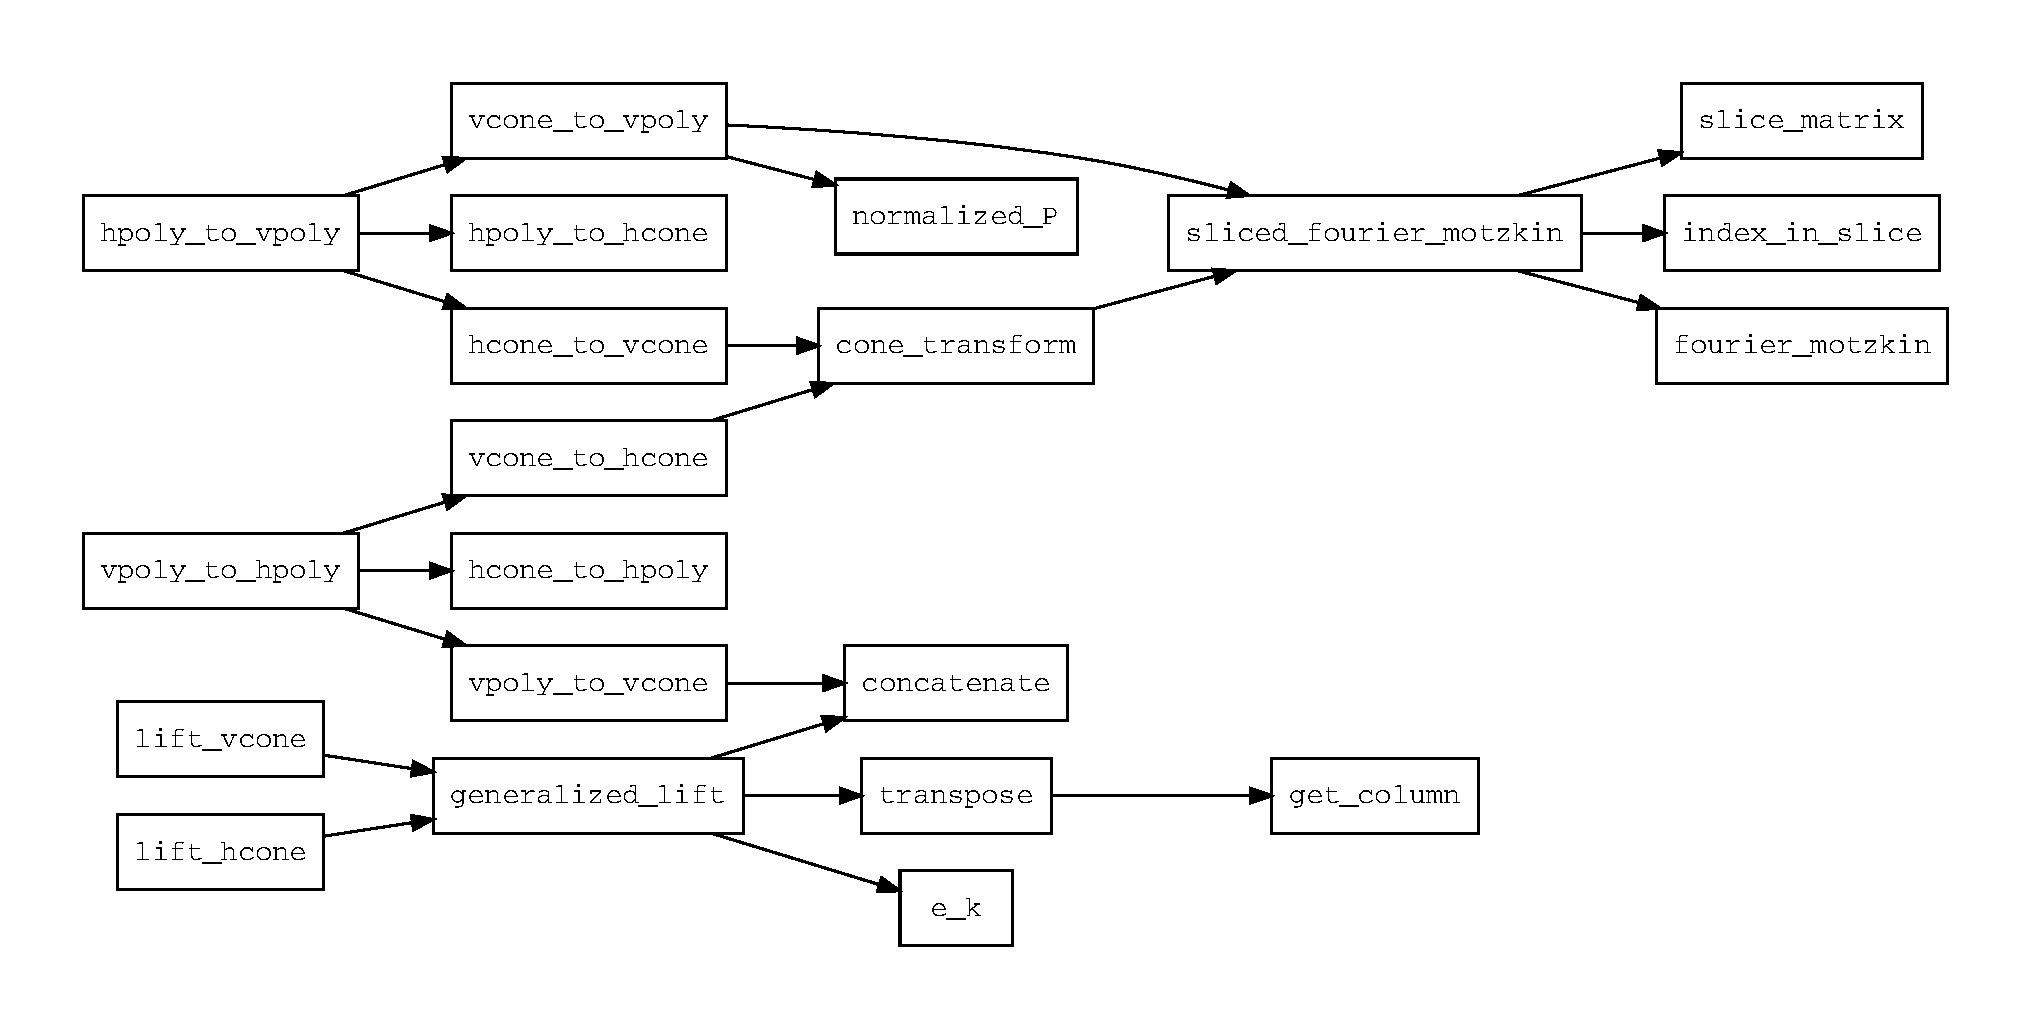
\includegraphics[keepaspectratio,width=\textwidth,height=\textheight]{../img/callgraph.pdf}


\chapter{Testing}

In the next sections, the methods used for testing the program described above will be discussed.

\paragraph{Notation:} Let $AU \leq \b$ be shorthand for $(\forall \u\in U) A\u \leq \b$.

\section{Testing H-Cone $\to$ V-Cone}
Suppose we have an H-Cone $C_A= \HC{A}$, and would like to test if a V-Cone $C_{V'} = \cone(V')$ represents the same set.  It's easy to check that
\[ AV'\leq\0 \Rightarrow C_{V'} \subseteq C_A\]
It's not clear what to do to check if $C_A\subseteq C_{V'}$.  Suppose we had a set $V$, and we knew that $C_A= \cone(V)$, and that $C_A= C_{V'} \Rightarrow V \subseteq V'$.  Then we'd have the following situation:
\begin{alignat*}{2}
	 & AV'\leq\0 \;      & \Rightarrow & \; C_{V'} \subseteq C_A \\
	 & V \subseteq V' \; & \Rightarrow & \; C_A\subseteq C_{V'}  \\
	 & C_{V'} = C_A \;   & \Rightarrow & \; V \subseteq V'       \\
	 & C_{V'} = C_A \;   & \Rightarrow & \; AV'\leq\0
\end{alignat*}

The problem is now to come up with such a set $V$.  We will need to relax the requirements on $V$ a little bit, but not in a way that reduces its utility.  The set is desribed in the next proposition, but first we introduce the notion of equivalence vectors:

\begin{Def}[vector equivalence]
	Let $\u,\v \in \R^d$, and suppose that $\u/\norm{\u} = \v/\norm{\v}$.  Then say that $\u,\v$ are equivalent, and write:
	\[ \u \simeq \v \]
\end{Def}

\begin{Def}[Extreme]
	Let $V \in \R^{d\times n}$.  $V$ is \textit{extreme} if, for any $\t\geq\0$ and $\v = V\e_k$, the following holds:
  \[V\t = \v \Rightarrow \t = \e_k \]
\end{Def}

\begin{Prop}\label{extreme_v}
	Let $V \in \R^{d\times n}$ be extreme, and $C = \cone(V)$.  Then
	\[ C = \cone(V') \Rightarrow (\forall \v \in V)(\exists \v'\in V') : \v \simeq \v' \]
\end{Prop}

\begin{proof}
	Let $\v \in V$, so that $\v = V\e_k$.  Since $C = \cone(V')$, there exists a matrix $A$ with all non-negative entries such that $V' = VA$.  There is also a non-negative $\b$ such that $\v = V'\b$.  Then $\v = (VA)\b = V(A\b)$.  Since $A$ and $\b$ contain only non-negative entries, so does $A\b$.  Since $V$ is extreme, $A\b$ must be the basis vector $\e_k$.  Then if $i \neq k$, $\e_i^T(A\b) = 0$, or $(\e_i^TA)\b = \sum_j A_i^j b_j = 0$.  Since $A_i^j, b_j \geq 0$, we have:
	\begin{alignat*}{3}
		(\forall i \neq k) & \quad & A_i^j > 0 \; & \Rightarrow & \; b_j = 0   \\
		(\forall i \neq k) & \quad & b_j > 0   \; & \Rightarrow & \; A_i^j = 0
	\end{alignat*}
	Furthermore, we have $\ip{A_k}{\b} = 1$, so for some $l$, $A_k^l,b_l > 0$.  Then,
	\[ (\forall i \neq k)\quad A_i^l = 0 \]
	Now let $\b'=\e_l/A_k^l$.  Then it immediately follows that $\ip{A_k}{\b'} = 1$.  Also,
	\[ (\forall i \neq k)\quad A_i^l = 0 \quad \Rightarrow\quad \ip{A_i}{\b'} = A_i^l/A_k^l = 0\]
	We conclude that $A\b' = \e_k = A\b$, and that $\v = V(A\b) = V(A\b') = (VA)\b' = U(\e_l/A_k^l)$.  If $\v' = U\e_l$, that is $\v'$ is the $l$-th vector of $U$, then $\v = \v'/A_k^l$, or
	\[ \v/\norm{\v} = (\v'/A_k^l)/\norm{\v'/A_k^l} = \v'/\norm{\v'} \]
	So $\v \simeq \v'$.
\end{proof}

Let's denote $(\forall \v \in V)(\exists \v'\in V') : \v \simeq \v'$ as $V \sqsubseteq V'$.  Then, considering the discussion before the proposition, we have the following result.

\begin{EqCriteria}[H-Cone $\to$ V-Cone]\label{eq_hc_vc}
	Say $V \in \R^{d\times n}$ is extreme, and let $C_A = \HC{A} = \cone(V)$.  Then
	\[ C_A = \cone(V') \;\Leftrightarrow\; AV'\leq\0,\, V \sqsubseteq V' \]
\end{EqCriteria}

\begin{Test}[H-Cone $\to$ V-Cone]\label{test_hc_to_vc}
	We now have a method for testing the program.  First, we hand-craft an H-Cone $\HC{A}$ based on some extreme set $V$, then run our program to get a set $V'$, with the alleged property that $\cone(V') = \HC{A}$.  If we confirm \Cref{eq_hc_vc}, then our program has succeeded.
\end{Test}

\subsection{Farkas Lemma}
The procedure for the other direction is \textit{almost} identical, but there is a slight catch.  Call a set of row vectors \textbf{extreme} if no row is a non-negative combination of the other.  We would be able to use \Cref{eq_hc_vc} to say something similar about an extreme set of row vectors $A$, if we could say that:

\begin{Thm}[Dual Cone]\label{dual_cone}
	\[ \HC{A} = \HC{A'} \Leftrightarrow \cone(A^T) = \cone(A'^T) \]
\end{Thm}

To prove this proposition, we use the Farkas Lemma:

\begin{Prop}[The Farkas Lemma]\label{farkas_lemma}
	Let $U \in \R^{d\times n}$.  Precisely one of the following is true:
	\[ (\exists \t \geq \0) : \x = U\t \]
	\[ (\exists \y) : U^T\y \leq 0,\; \ip{\x}{\y} > 0 \]
\end{Prop}

\begin{proof}  That both can't be true can be seen by:
	\[ \x = U\t \quad\Rightarrow\quad \y^T\x = \y^T U\t \quad\Rightarrow\quad 0 \neq 0 \]
	To see that at least one is true we must reconsider the process of converting a V-Cone to an H-Cone.  First, from $\cone(U)$ we create the following matrix:
	\[ A = \begin{pmatrix*}[r] \0 & -I \\ I & -U \\ -I & U \end{pmatrix*}  \]
	By the way $A$ is constructed,
	\begin{equation}\label{eq:flcone}
		(\exists \t) : A \xt \leq \0 \Leftrightarrow (\exists \t\geq\0)\; \x = U\t
	\end{equation}
	In the proof of the transformation, we use \Nameref{fm_hcone} to transform that matrix $A$.  The \Nameref{fm_matrix} promises a sequence of matrices $Y_{d+1}, \dots, Y_{d+n}$ with certain properties.  Let $Y = (Y_{d+n})(Y_{d+(n-1)})\dots(Y_{d+1})$, then it can be said of $Y$:
	\begin{enumerate}
		\item Every element of $Y$ is non-negative.
		\item $Y$ is finite.
		\item The last $n$ columns of $YA$ are all $\0$.
		\item \((\exists t_{d+1},\dots,t_{d+n})A(\x + \sum_{i=d+1}^{d+n} t_i\e_i) \leq \0
		      \Leftrightarrow (YA)\x \leq \0 \)
	\end{enumerate}
	Note that here $\x \in \R^{d+n}$.  $A$ has three blocks of rows, which can be labeled with $Z,P,N$ in a fairly obvious way.  Then, $Y$ can be broken up into three blocks of columns, so that
	\[ Y = (Y_Z \; Y_P \; Y_N) \]
	Where each of $Y_Z,Y_P,Y_N \geq \0$.  Consolidating what is known about $A$ and $Y$,
	\[ YA = (Y_Z \; Y_P \; Y_N) \begin{pmatrix*}[r] \0 & -I \\ I & -U \\ -I & U \end{pmatrix*}
		= (Y' \; \0) \]
	Here, we have let $Y' = Y_P - Y_N$.  Then it follows that
	\[ \0 = -Y_Z - Y_P(U) + Y_N(U) = -Y_Z - Y'(U) \;\Rightarrow\; Y_Z = - Y'U
		\;\Rightarrow\; Y'U \leq \0 \]
	Then it holds that, for any row $\y' \in Y'$:
	\begin{equation}\label{eq:flneg}
		\y'U \leq \0
	\end{equation}
	It is also true that
	\[ (YA)\xt = (Y'\;\0)\xt = Y'\x \]
	We also have
	\begin{equation}\label{eq:flconst}
		(\exists \t) : A \xt \leq \0 \Leftrightarrow
		(YA)\xt \leq \0 \Leftrightarrow
		Y'\x \leq \0
	\end{equation}
	Note that here $\x \in \R^d$.  So, if given some $\x$, the left side of \eqref{eq:flconst} is not satisfied, then neither is the right, and there must be some row $\y' \in Y'$ such that the following holds:
	\begin{equation}\label{eq:flconstbrk} \ip{\y'}{\x} > 0 \end{equation}
	Then we conclude that, if the right side of \eqref{eq:flcone} fails, then there is a vector $\y' \in Y'$ satisfying \eqref{eq:flneg} and \eqref{eq:flconstbrk}.
\end{proof}

\section{Testing V-Cone $\to$ H-Cone}

Now we can prove \nameref{dual_cone}:
\[ \HC{A} = \HC{A'} \Leftrightarrow \cone(A^T) = \cone(A'^T) \]

\begin{proof}
	First suppose that $\cone(A^T) = \cone(A'^T)$.  Then there exists a non-negative matrix $B$ such that $A'^T = A^TB$.  Then $A\x \leq \0 \Rightarrow B^TA\x\leq \0 \Rightarrow A'\x\leq\0$.  Precisely the same reasoning shows that $A'\x\leq\0 \Rightarrow A\x\leq\0$, and we conclude that $\cone(A^T) = \cone(A'^T) \Rightarrow \HC{A} = \HC{A'}$.

	Next suppose that $\cone(A^T) \neq \cone(A'^T)$, that is, let $\z \in \cone(A), \z \not\in\cone(A')$.  We must show that $\HC{A} \neq \HC{A'}$.  By the Farkas Lemma, we have a $\y$ such that $\ip{\y}{\z} > 0,\; A'\y \leq \0$.  Clearly this means that $\y \in \HC{A'}$.  Since $\z \in \cone(A)$, there is some $(\t \geq \0): \z^T = \t^T A$.  Then if $A\y\leq\0$, we would have $\ip{\y}{\z} = \t^T A\y \leq 0 < \ip{\y}{\z}$, a contradiction.  So we conclude that $\y\not\in\HC{A}$.
\end{proof}

Now, as before, we suppose that we have a set $V$ and $A$, where $A$ is extreme, and we know that $C = \cone(V) = \HC{A}$.  We have the following situation:
\begin{alignat*}{2}
	 & C = \HC{A'}    \;   & \Rightarrow & \; A \sqsubseteq A'    \\
	 & C = \HC{A'}    \;   & \Rightarrow & \; A'V\leq\0           \\
	 & A \sqsubseteq A' \; & \Rightarrow & \; \HC{A'} \subseteq C \\
	 & A'V\leq\0  \;       & \Rightarrow & \; C \subseteq \HC{A'}
\end{alignat*}
So we have the following.

\begin{EqCriteria}[V-Cone $\to$ H-Cone]\label{eq_vc_hc}
	Let $A\in\R^{m\times d}$ be extreme, and $C_V = \cone(V) = \HC{A}$.  Then
	\[ C_V = \HC{A'} \;\Leftrightarrow\; A'V\leq\0,\; A \sqsubseteq A' \]
\end{EqCriteria}

\begin{Test}[V-Cone $\to$ H-Cone]\label{test_vc_to_hc}
	We now have a method for testing the program.  First, we hand-craft an V-Cone $\cone{V}$ based on some extreme set $A$, then run our program to get a set $A'$, with the alleged property that $\cone(V') = \HC{A}$.  If we confirm \Cref{eq_vc_hc}, then our program has succeeded.
\end{Test}

\section{Testing H-Polyhedron $\to$ V-Polyhedron}

Say we have an H-Polyhedron $P_{A,\b} = \HP{A}{\b}$, and wish to check that our program correctly calculates a $V'$ and $U'$ such that $P_{A,\b} = \VP{U'}{V'}$.  Again, we shall use the notion of extremity and show that under certain circumstances we can use extreme sets to demonstrate the validity of our algorithm.  In this case, the definition of extreme is a little more complicated, but it asserts that a set $U$ is extreme as before, and that no element of another set $V$ can be expressed as a non-trival sum of a convex combination of $V$ and a non-negative linear combination of members of $U$.

\begin{Def}[Extreme Pair]{ A pair of sets $U\in\R^{d\times n}, V\in\R^{d\times p}$ is called an \textit{extreme pair} if for any $\u = U\e_k, \v = V\e_l$ the following is true:
		\begin{alignat*}{1}
			 & \t \geq \0,\; \u = U\t \Rightarrow \t = \e_k                              \\
			 & \t \geq \0, \blambda \geq \0, \ip{\blambda}{\1} = 1, \v = U\t + V\blambda
			\Rightarrow \t = \0, \blambda = \e_l
		\end{alignat*}
	}\end{Def}

Let us now consider the set $U$ in the expression $\HP{A}{b} = \VP{U}{V}$.

\begin{Prop}[Characterstic Cone]\label{characteristic_cone}
	Suppose that $P = \HP{A}{b} = \VP{U}{V}$.  Then
	\[ \cone(U) = \HC{A} \]
\end{Prop}

\begin{proof}
	We show that the following three statements are equivalent:
	\begin{enumerate}
		\item $A\r\leq\0$
		\item $(\forall \x\in P)(\forall \alpha > 0)\;\x + \alpha\r \in P$
		\item $\r \in \cone(U)$
	\end{enumerate}
	$(1 \Rightarrow 2)$. $\x\in P$ means that $A\x\leq\b$, and $A\r\leq\0$ means that $A(\x+\alpha\r) \leq A\x \leq \b$.\\
	$(\neg 1 \Rightarrow \neg 2)$.  Suppose $\ip{A_i}{\r} > 0$, then let $\alpha > (b_i - \ip{A_i}{\x})/\ip{A_i}{\r}$.  We have:
	\[ \ip{A_i}{\x + \alpha\r} > \ip{A_i}{\x} +
		\frac{b_i\ip{A_i}{\r} - \ip{A_i}{\x}\ip{A_i}{\r}}{\ip{A_i}{\r}} = b_i \]
	$(3 \Rightarrow 2)$.  This is essentially the definition of $\VP{U}{V}$.\\
	$(2 \Rightarrow 3)$.  Now for the real work.  Suppose that (2) holds, but $\r\not\in\cone(U)$.  Then by the Farkas Lemma, we have a $\y$ that satisfies $(\forall \r\in U)\,\ip{\r}{\y}\leq 0,\; \ip{\y}{\r} > 0$.  From (2) we construct a sequence: $(\x_n) = \v+n\cdot\r$.  Then it is clear that the sequence $\ip{\y}{\x_n} \to \infty$.  It is also clear that $(\forall n)\,\x_n \in P$.  We now need the following:
	\begin{itemize}
		\item A linear, real-valued function on the set $\conv(V)$ achieves its maximal value at some $\bar\v \in V$.
	\end{itemize}
	To see this is true, suppose that the linear function is given by $\ip{\y}{\cdot}$, and that $\bar\v$ is an element of $V$ such that $(\forall \v \in V)\,\ip{\y}{\bar\v} \geq \ip{\y}{\v}$.  Then, for any $\r \in \conv(V)$, $\r = \sum_{\v\in V} \lambda_v\v$ where $\sum \lambda_v = 1 \Rightarrow \lambda_v \leq 1$, and it follows
	\[\ip{\y}{\r} = \ip{\y}{\sum_{\v\in V}\lambda_v v} = \sum_{v\in V} \lambda_v\ip{\y}{\v}
		\leq \sum_{v\in V}\lambda_v\ip{\y}{\bar\v} = \ip{\y}{\bar\v} \]
	Now consider the maximum value of the function $\ip{\y}{\cdot}$ on $P$.  Since any element of $P$ can be written $\r + \v \st \r\in\cone(U),\,\v\in\conv(V)$, and $(\forall\r\in U) \ip{\y}{\r} \leq 0$, we can find the maximum value on $\conv(V)$.  However, $\ip{\y}{\cdot}$ achievs its maximal value on $\conv(V)$ at some $\bar\v\in V$, which is a contradiction with the fact that $\ip{\y}{\x_n} \to \infty$, so we conclude that $\r\in\cone(U)$.
\end{proof}

\begin{Remark}[Characteristic Cone]\label{characteristic_cone}  Note that $(2)$ in the proof above is independent of $A$ and $U$.  This means that the cone of a polyhedron is independent of its representation, i.e. if $\VP{U}{V} = \VP{U'}{V'}$, then $\cone(U) = \cone(U')$, while it is not necessarily true that $\conv(V) = \conv(V')$.  Similarly, if $\HP{A}{\b} = \HP{A'}{\b'}$, the it holds that $\HC{A} = \HC{A'}$.
\end{Remark}

\begin{Prop}\label{conv_conv}
	A convex combination of convex combinations is another convex combination
\end{Prop}
\begin{proof}
	Let $\Lambda$ represent a collection of convex combinations, that is, $\vec{1}^T\Lambda = \vec{1}^T$, and let $\blambda\geq\0,\,\1^T\blambda = 1$ be a convex combinator.  Then $\Lambda\blambda = \blambda'$ where $\blambda'\geq\0,\,\1^T\blambda'=1$.  That $\blambda'\geq\0$ is clear, then just note that $\1^T\blambda' = \1^T\Lambda\blambda = \1^T\blambda = 1$.
\end{proof}

\begin{Prop}[Minkowski Sums]\label{minkowski_formula}
	The following two statements hold
	\begin{enumerate}
		\item $A \subseteq B, C\subseteq D \Rightarrow A + C \subseteq B + D$
		\item $P + \cone(U) + \cone(U) = P + \cone(U)$
	\end{enumerate}
\end{Prop}

\begin{proof}
	(1) $a\in A \Rightarrow a\in B,\; c\in C\Rightarrow c\in D$.  Taken together, $a+c \in B+D$.\\
	(2) $\t,\t'\geq\0 \Rightarrow p + U\t + U\t' = p + U(\t+\t') = p + U\t'', \t''\geq\0$.
\end{proof}

\begin{EqCriteria}\label{eq_hp_vp}
	Suppose that there is an extreme pair $U,V$ such that $P_{A,\b} = \HP{A}{b} = \VP{U}{V}$.  Then the following are equivalent:
	\begin{enumerate}
		\item $P_{A,\b} = \VP{U'}{V'}$
		\item $U \sqsubseteq U',\; V \subseteq V',\; AU'\leq\0,\, AV'\leq\b$
	\end{enumerate}
\end{EqCriteria}

\begin{proof}
	$(2 \Rightarrow 1)$.  There's not too much to say about this direction, it's mostly just collecting some straightforward observations and results.
	\begin{itemize}
		\item[(a)] $U \sqsubseteq U' \Rightarrow \cone(U) \subseteq \cone(U')$
		\item[(b)] $V \subseteq V' \Rightarrow \conv(V) \subseteq \conv(V')$
		\item[(c)] (a) + (b) $\Rightarrow P_{A,\b} \subseteq \VP{U'}{V'}$
		\item[(d)] $AU'\leq\0 \Rightarrow \cone(U') \subseteq \cone(U)$
		\item[(e)] $AV'\leq\b \Rightarrow \conv(V') \subseteq P_{A,\b}$
		\item[(f)] (d) + (e) $\Rightarrow \VP{U'}{V'} \subseteq P_{A,\b} + \cone(U) = P_{A,\b}$
		\item (c) + (f) $\Rightarrow (2 \Rightarrow 1)$
	\end{itemize}
	(a) and (b) are clear, (c) uses \Cref{minkowski_formula}, (d) requires \nameref{characteristic_cone}, (e) is clear, and (f) uses \Cref{minkowski_formula}.

	$(1 \Rightarrow 2)$.  This direction is a little more interesting.  First we observe:
	\[ \cone(U) = \HC{A} = \cone(U') \Rightarrow U \sqsubseteq U' \]
	The equalities follow from \nameref{characteristic_cone}, and the implication follows from \Cref{eq_hc_vc}.  Note that the extremeness of $U$ and the Farkas lemma are both used here.  Since we know that $\cone(U) = \cone(U')$, we also know that $\VP{U'}{V'} = \VP{U}{V'}$.  Next, we consider $V$ and exploit its extremeness.  Since $P_{A,\b} = \VP{U}{V'}$, each $\v'\in V'$ can be written $U\t + V\blambda$, where $\t \geq \0$ and $\blambda$ is a convex combinator.  We combine these into matrices $T$ and $\Lambda$, so $V' = UT + V\Lambda$.  But it is also true that every $\v\in V$ can be written as
	\[ \v = U\t + V'\blambda = U\t + (UT + V\Lambda)\blambda = U\t' + V\blambda' \]
	Where $\t'\geq\0$, and $\blambda'$ is a convex combinator.  Because $U,V$ is an extreme pair, we have that $\t'=\0$, and $\blambda = \e_k$ for some $k$.  Because $U$ is extreme, it does not contain $\0$, and so $\t = \0$.  This puts us at $\v = V'\blambda = V\Lambda\blambda = V\blambda'$, and $\blambda' = \e_k$.  In order that $\blambda' = \e_k$, for every column of $\Lambda$ corresponding to a positive entry in $\blambda$, only one row may contain a positive entry, and that entry must be $1$.  Then instead of $\blambda$, use instead $\e_l$ where $\Lambda_k^l = 1$.  Then $\Lambda\blambda = \Lambda\e_l$, so $V\Lambda\blambda = V\Lambda\e_l = V'\e_l=\v'$ where $\v'\in V'$.  Then $\v \in V'$.

	That $AV'\leq\b$ is obvious, and that $AU'\leq\0$ is mentioned in the remarks after \Cref{characteristic_cone}.
\end{proof}

\begin{Test}[H-Polyhedron $\to$ V-Polyhedron]\label{test_hp_to_vp}
	We now have a method for testing the program.  First, we hand-craft an H-Polyhedron $\HP{A}{\b}$ based on some extreme pair $(U,V)$, then run our program to get the pair $(U',V')$, with the alleged property that $\HP{A}{\b} = \VP{U'}{V'}$.  If we confirm \Cref{eq_hp_vp}, then our program has succeeded.
\end{Test}

\section{Testing V-Polyhedron $\to$ H-Polyhedron}
Now we suppose we have a V-Polyhedron $P_{U,V} = \VP{U}{V}$, and would like to test the program which returns a matrix-vector pair $A',\b'$ where supposedly $P_{U,V} = \HP{A'}{\b'}$.  Again, we will start off with a pair $A,\b$ where we know that $P_{U,V} = \HP{A}{\b}$, where $A,\b$ satisfy some nice properties, and use those properties to test if $P_{U,V} = \HP{A'}{\b'}$.  In order to demonstrate these properties, the Farkas Lemma will be used, but in different forms.  We want to use \Cref{eq_vc_hc}, but first we have to check:

\begin{Prop}\label{homogenization_cone}
	The following statements are equivalent:
	\begin{enumerate}
		\item $\HP{A}{\b} = \HP{A'}{\b'}$
		\item $\set{\xx \big| \pmb -1 & \0 \\ -\b & A \pme \xx \leq \0} =
			      \set{\xx \big| \pmb -1 & \0 \\ -\b' & A' \pme \xx \leq \0}$
	\end{enumerate}
\end{Prop}

\begin{proof}
	$(2 \Rightarrow 1)$.  Just set $x_0 = 1$, and move $\b,\b'$ to the right side of the inequalities.
	$(\neg 2 \Rightarrow \neg 1)$.  Suppose that:
	\[ \pmb -1 & \0 \\ -\b & A \pme \xx \leq \0,\quad
		\pmb -1 & \0 \\ -\b' & A' \pme \xx \not\leq \0 \]
	Observe that, by the way these sets are constructed, $x_0 \geq 0$.  If $x_0 = 0$, then we have $\HC{A} \neq \HC{A'}$, which, by the remark following \Cref{characteristic_cone} means that $\HP{A}{\b} \neq \HP{A'}{\b'}$.  If $x_0 > 0$, then we have:
	\[ A\x \leq x_0\b,\;A'\x\not\leq x_0\b' \Rightarrow A(\x/x_0)\leq\b,\;A'(\x/x_0)\not\leq\b' \]
	So $\HP{A}{\b} \neq \HP{A'}{\b'}$.
\end{proof}

Now, combining the results of \Nameref{characteristic_cone} and \cref{homogenization_cone}, we have the following result:

\begin{Prop}\label{dual_homogenization_cone}
	The following two statement are equivalent:
	\begin{enumerate}
		\item $\HP{A}{\b} = \HP{A'}{\b'}$
		\item $\cone \pmb -\b^T & -1 \\ A^T & \0 \pme = \cone \pmb -\b'^T & -1 \\ A'^T & \0 \pme$
	\end{enumerate}
\end{Prop}
%\begin{proof} This immediately follows from propositions \ref{homogenization_cone} and \ref{dual cone}.  \end{proof}

\subsection{Extreme H-Polyhedra Pairs}
\begin{Def}[Extreme Pair]{
		A pair $A,\b$ is called \textbf{extreme} if $\HP{A}{\b}$ is non-empty, and
		\[ \t \geq \0,\, \t^T(A,b) = (A_i,b_i) \Rightarrow [\t \neq \0 \Rightarrow \t = \e_i] \]
	}\end{Def}

Of course, we want to say that if $P = \HP{A}{\b}$ where $(A,\b)$ is an extreme pair, and $P = \HP{A'}{\b'}$, then, by \Cref{dual_homogenization_cone}, $(A,\b) \sqsubseteq (A',\b')$.  The catch is that the cones in \Cref{dual_homogenization_cone} have a strange form.  What we want to be true turns out to be so, but before we can prove this fact, we need a property of extreme pairs, which requires a new form of the Farkas Lemma.

\subsection{Farkas Lemma: Round 2}

Let us restate the conclusion of the Farkas Lemma:
\newcommand{\xor}{\;\Leftrightarrow\;\neg}
\[ \exists \t\geq\0 \st U\t = \x \xor \exists \y\st \y^TU\leq\0,\, \y^T\x > 0 \]
If we let $U = (A,-A,I)$, and  we get a new form:
\[ \exists \t \geq\0 \st (A,-A,I)\t = \x \xor \exists \y\st \y^T(A,-A,I)\leq\0,\, \y^T\x > 0 \]
Then breaking apart $\t = (\t_P,\t_N,\t_I)$, we have
\[ (A,-A,I)\pmb \t_P\\ \t_N\\ \t_I \pme = \x \Rightarrow A(\t_P - \t_N) = \x - \t_I \]
If we let $\t_P - \t_N = \z$, then $\z$ is no longer constrained by $\t \geq\0$, and we have that $A\z \leq \x$.  Since $\y^T A \leq \0$ and $-\y^T A\leq \0$, it must be that $\y^T A = \0$.  Combining these results, relabeling $\x$ as $\b$ and $\z$ as $\x$, and $\y$ as $-\y$, we see a new form of Farkas Lemma:
\begin{Thm}[Farkas Lemma 2]\label{FL2}
	\[ \exists \x \st A\x \leq \b \xor \exists \y\geq\0 \st \y^TA = \0,\, \y^T\b < 0 \]
\end{Thm}
This form tells us that an H-Polyhedron is non-empty, or we can create an inequality that is impossible to solve from it's matrix.  The next form shows a similar result, but this time it is for a specific $\x$, not implying the emptyness of the Polyhedra, just the constraints' failure to be satisfied at a specific point.
%
%First observe that (using \eqref{FL2})
%\[ A\x \not\leq \b \Leftrightarrow \neg \exists \z\st
%	\pmb A\\I\\-I\pme \z \leq \pmb \b\\ \x\\ -\x \pme \Leftrightarrow
%	\exists \y\geq\0\st \y^T\pmb A\\I\\-I\pme =\0,\, \y^T\pmb \b\\ \x\\ -\x \pme < 0\]
%Splitting up $\y$ into components like we did before with $\t$, we can rewrite this as
%
%\begin{equation} \label{eq:FL3}
%	A\x \not\leq \b \Leftrightarrow \exists \y\st \y^T A = \w,\, \y^T \b < \w^T\b
%\end{equation}

We can now prove some useful properties of extreme pairs.

\begin{Prop}\label{extreme_Ab_pair_properties}
	Let $A,\b$ be an extreme pair.  Then the following holds:
	\begin{alignat*}{6}
		\t\geq\0,\,\t^T A \, & = & \, \0  \, & \Rightarrow & \, [\t & \neq & \, \0 \,   & \Rightarrow & \, \ip{\t}{\b} \, & > & \, 0 ]   \\
		\t\geq\0,\,\t^T A \, & = & \, A_i \, & \Rightarrow & \, [\t & \neq & \, \e_i \, & \Rightarrow & \, \ip{\t}{\b} \, & > & \, b_i ]
	\end{alignat*}
\end{Prop}

\begin{proof}
	Suppose that $\t^T A = \0,\, \t\neq\0$.  Next suppose that $\ip{\t}{\b} = 0$.  Then $(\t + \e_i)(A,b) = (A_i,b_i)$, but $\t+\e_i \neq \e_i$, a contradiction.  Next suppose that ${\ip{\t}{\b} < 0}$.  Then we have that $\exists \t\geq\0,\,\t^T A = \0,\,\t^T \b < 0$, which by \nameref{FL2} means that $\HP{A}{b}$ is empty, a contradiction.  So the first property is proven.

	Now suppose that $\t^T A = A_i, \t\neq\e_i$.  Then we know that $\t^T \b \neq b_i$, but if $\ip{\t}{\b} < 0$, we'd have that $(\t - \e_i)^T A = \0, (\t-\e_i)^T\b < 0$, contradicting the first property.
\end{proof}

We are now prepared to prove the following proposition.

\begin{Prop}\label{extreme_Ab}
	Suppose that $\HP{A}{\b} = \HP{A'}{\b'}$, where $(A,\b)$ is an extreme pair.  Then $(A,\b) \sqsubseteq (A',\b')$.
\end{Prop}

\begin{proof}
	It suffices to show that $\pmb -\b^T & -1 \\ A^T & \0 \pme$ is extreme, for then:
	\[\pmb -\b^T & -1 \\ A^T & \0 \pme \sqsubseteq \pmb -\b'^T & -1 \\ A'^T & \0 \pme \Rightarrow
		\pmb -\b^T \\ A^T \pme \sqsubseteq \pmb -\b'^T \\ A'^T \pme \Rightarrow
		(A,\b) \sqsubseteq (A',\b')
	\]
	So, suppose that $(\t,t) \geq \0$, $\pmb -\b^T & -1 \\ A^T & \0 \pme(\t,t) = \pmb -b_i \\ A^T_i\pme$.  We must show that $\t = \e_i$, $t = 0$.  Suppose that it's not.  Then we have $\t^T A = A_i$, and by \Cref{extreme_Ab_pair_properties} $\ip{\t}{-\b} < b_i$.  Since $-t \leq 0$, $\ip{\t}{-\b} - t < b_i$, a contradiction.  So we have shown that $\t = \e_i$, in which case $t = 0$, and the proposition follows.
\end{proof}

Suppose that we have a $(U,V)$ and $(A,\b)$ such that $P_{UV} = \VP{U}{V} = \HP{A}{\b}$, and $(A,\b)$ is an extreme pair.  We run our program and get a new pair $(A',\b')$.  Denote $P_{A',\b'} := \HP{A'}{\b'}$.  We would like to verify that $P_{UV} = P_{A',\b'}$.  We have the following:
\begin{alignat*}{2}
	 & A'U\leq\0,\, A'V\leq\b'     & \;\Rightarrow\; & P_{UV} \subseteq P_{A',\b'}  \\
	 & (A,\b) \sqsubseteq (A',\b') & \;\Rightarrow\; & P_{A',\b'} \subseteq P_{UV} \\
	 & P_{UV} = P_{A',\b'}         & \;\Rightarrow\; & A'U\leq\0,\, A'V\leq\b'      \\
	 & P_{UV} = P_{A',\b'}         & \;\Rightarrow\; & (A,\b) \sqsubseteq (A',\b')
\end{alignat*}
The last line uses \Cref{extreme_Ab}.  So we conclude:

\begin{EqCriteria}\label{eq_vp_hp}
Suppose that there is an extreme pair $(A,\b)$ such that $P_{UV} = \VP{U}{V} = \HP{A}{b}$.  Then the following are equivalent:
\[ P_{UV} = \HP{A'}{\b'} \Leftrightarrow A'U\leq\0,\,A'V\leq\b',\,(A,\b)\sqsubseteq (A',\b') \]
\end{EqCriteria}

\begin{Test}[V-Polyhedron $\to$ H-Polyhedron]\label{test_vp_to_hp}
	We now have a method for testing the program.  First, we hand-craft a V-Polyhedron $\VP{U}{V}$ based on some extreme pair $(A,\b)$, then run our program to get the pair $(A',\b')$, with the alleged property that $\VP{U}{V} = \HP{A'}{\b'}$.  If we confirm \Cref{eq_vp_hp}, then our program has succeeded.
\end{Test}

\section{\filename{test\_functions.h}}

The following types are defined for running tests of the different algorithms.  They are expected to be given a descriptive name, the object on which the test will be run, and a \lsti{key} with which the result of the test will be compared.  The \lsti{key} object is one of the extreme objects described above.
\lsthconetestcasea
\lstvconetestcasea
\lsthpolytestcaseb
\lstvpolytestcaseb

\section{\filename{test\_functions.cpp}}

The dot-product and norm (in terms of dot product).
\lstoperator
\lstnorm

\lsti{approximately_zero} is used during tests to avoid issues involving floating point rounding errors.  For example, \lsti{1/6.0 * 2.5 - 5/12.0 == 0} will give \lsti{false}, while \lsti{approximately_zero(1/6.0 * 2.5 - 5/12.0)} will return \lsti{true}.  Test cases are used where intermediate calculations don't depend on such high accuracy, and these discrepencies can be ignored.

\lsti{approximately_zero(c) == true} is be denoted $\mli{c} \approx 0$.
\lstapproximatelyzeroa

Tests $c < 0 \lor c \approx 0$.
\lstapproximatelyltzero

Tests $\norm{\v} \approx 0$.  This is be denoted $\v \approx \0$.
\lstapproximatelyzerob

Tests $\u/\norm{\u} - \v/\norm{\v} \approx \0 $.  This is be denoted $\u \simeq \v$.
\lstisequivalent

Tests $\u - \v \approx \0$.  This is be denoted $\u \approx \v$.
\lstisequal

Tests $(\exists \u \in U) \st \v \simeq \u$.
\lsthasequivalentmember

Tests $(\exists \u \in U) \st \v \approx \u$.
\lsthasequalmember

Tests $(\forall v \in V)(\exists \u \in U) \st \v \simeq \u$.  This is be denoted $V \sqsubseteq U$.
\lstsubsetmodeq

Tests $(\forall v \in V)(\exists \u \in U) \st \v \approx \u$.  This is be denoted $V \subseteq U$.
\lstsubset

Given a \mli{Vector constraint} and \mli{Vector ray}, tests if \\
\lsti{approximately_lt_zero(ray * constraint)}.  Note that if the constraint is of the form $\ip{A_i}{\v} \leq b$ for some value $b$, then this tests $\ip{A_i}{\mli{ray}}\leq\0$.
\lstraysatisfieda

Test $A\v \leq \0$
\lstraysatisfiedb

Test $AV \leq \0$
\lstrayssatisfied

Test $\ip{A_i}{\v} \leq b_i$
\lstvecsatisfieda

Test $A\v \leq \b$
\lstvecsatisfiedb

Test $AV \leq \b$
\lstvecssatisfied

Given an H-Cone $C = \HC{A} = \cone(U)$ where $U$ is extreme, and a \lsti{Matrix} $U'$, determines if $C = \cone(U')$.
Similarly, given a V-Cone $C = \cone(U) = \HC{A}$ where $A$ is extreme, and a \lsti{Matrix} $A'$, determines if $C = \HC{A'}$.
\lstequivalentconerep

Given an H-Polytope $P = \HP{A}{\b} = \VP{U}{V}$ where $U$ and $V$ are extreme, and a pair $(U',V')$, determines if $P = \VP{U'}{V'}$.
\lstequivalenthpolyrep

Given a V-Polytope $P = \VP{U}{V} = \HP{A}{\b}$ where $A$ is extreme, and a \lsti{Matrix} $(A',\b')$, determines if $P = \HP{A'}{\b'}$.
\lstequivalentvpolyrep

%\lsthconetestcaseb
%\lstvconetestcaseb
%\lsthpolytestcasea
%\lstvpolytestcasea




%\chapter*{Conclusion}
\addcontentsline{toc}{chapter}{Conclusion}

In this thesis we have shown the proof of the \MWT.  The proof is constructive in nature, showing how to create the sets promised by the theorem, and a basic implementation is given.  While the proof is hardly elegant, it does show that the intutive result of the theorem is true by brute force methods and does not require any advanced results.  Indeed, the proof is from first principles, using the language of linear algebra.

The more interesting (and, perhaps, informative) part of the paper deals with creating a testing framework for the program.  This presented an opportunity to discuss pointed and full-dimensional polyhedra, and their relation to minimal and essential representations of polyhedra.  The characterstic and dual cones were defined with some useful properties proven, invoking the Farkas Lemma in a few different forms.  As of now, the testing framework is open for extension, to include polyhedra for which minimal representations are not guaranteed.

It may be worth mentioning an anachranism presented in the text.  The chapter on testing starts off by describing some sets that are chalked up to ``wishful thinking,'' then minimality is introduced and the useful properties are derived.  In earnest, the actual progression from wishful thinking to effective testing was a bit different.  Initially, the requirements for testing were received.  Then, the first idea was to create some cones, and check if one representation was a subset of another (modulo scaling, i.e. equivalence).  This is the simplest, most immediate (and perhaps natural) answer to the challenge for testing.  After this method was decided upon, the question then arose: ``what properties of the sets representing the polyhedra are necessary to ensure the tests will work?''  Then the properties were determined.  It was only afterwards that it became clear that these properties were actually pointed-ness and full-dimensionality, at which point the presenation was altered to emphasize this.  Without this alteration, the presentation would be akin to: ``these seemingly arbitrary properties allow us to test the polyhedra in this manner,'' which is much less nice than ``these natural classes of polyhedra have useful properties which allow us to test our implemenation on them.''

It should also be mentioned that the algorithm here is not efficient.  The intermediate represenations of the polyhedra may be exponential in the size of the input and output.  The ``double description'' method is a far better way to calculate the alternative representations desired, however the method is a bit more advanced and is better pursued after getting a decent grasp of the underlying problem.

The Farkas Lemma should have the last word, as it is a rather wonderful combinatorial compactification of much of the information of the \MWT.  It's main contribution here was to show that minimal sets of H-Polyhedra do exist, and then allowed us to re-use some of the work we had done with V-Polyhedra to expedite the proofs of the testing methods.


%%% Bibliography
\include{bibliography}

%%% Figures used in the thesis (consider if this is needed)
%\listoffigures

%%% Tables used in the thesis (consider if this is needed)
%%% In mathematical theses, it could be better to move the list of tables to the beginning of the thesis.
%\listoftables

%%% Abbreviations used in the thesis, if any, including their explanation
%%% In mathematical theses, it could be better to move the list of abbreviations to the beginning of the thesis.
%\chapwithtoc{List of Abbreviations}

%%% Attachments to the bachelor thesis, if any. Each attachment must be
%%% referred to at least once from the text of the thesis. Attachments
%%% are numbered.
%%%
%%% The printed version should preferably contain attachments, which can be
%%% read (additional tables and charts, supplementary text, examples of
%%% program output, etc.). The electronic version is more suited for attachments
%%% which will likely be used in an electronic form rather than read (program
%%% source code, data files, interactive charts, etc.). Electronic attachments
%%% should be uploaded to SIS and optionally also included in the thesis on a~CD/DVD.
%%% Allowed file formats are specified in provision of the rector no. 72/2017.
\appendix
%\chapter{Attachments}

%\section{First Attachment}

 \begin{thebibliography}{9}

 \bibitem{ziegler95}
   {\sc Ziegler,} Gunter.
   \emph{Lectures on Polytopes}.
   Springer-Verlag, New York, 1995.
   ISBN 0-387-94329-3.

 \end{thebibliography}

\openright
\end{document}
